\documentclass[titlepage,a4paper,11pt]{report}

\usepackage[utf8]{inputenc}
\usepackage[OT1]{fontenc}

\usepackage{illcmolthesis}

% put your own adjustments into headers.tex
\input{headers}

\begin{document}

\title{TITLE OF THE THESIS}
\author{Mees~Lürsen}
% \birthdate{April 1st, 1980} % optional
% \birthplace{Alice Springs, Australia} % optional
\defensedate{August 28, 2005}
\supervisor{Dr Erman Acar}
\committeemember{Dr Jack Smith}
\committeemember{Prof Dr Jane Williams}
\committeemember{Dr Jill Jones}
\committeemember{Dr Albert Heijn}
\maketitle

\begin{abstract}
  ABSTRACT OF THE THESIS

\end{abstract}

% If you want to, add acknowledgements *after* your defense.
% Do not add acknowledgements when you upload to DataNose.
% \begin{acknowledgements}
% \end{acknowledgements}

\clearpage

\tableofcontents

\chapter{Introduction}


\chapter{Background and Preliminaries}
    \section{Symbollic Regression}

    \section{Linear Temporal Logic with Finite Trace Semantics}
    
    \section{Many Syntaxes, One Semantics}

    \section{Kernel Methods}\label{sec:kernel_methods}
    
    % =====================================================================
    %  PRELIMINARIES SCAFFOLD — CE & RL machinery (general, citable only)
    %  Method-specific content (Hamming reward, hybrid loss, RB/GAE variants,
    %  Delta-z derivations, subset proof) is deferred to Ch.6 / appendix.
    % =====================================================================

    \section{Language Models, Self-Attention, and Cross-Attention}
    % Architecture already covered here; the items below add HOW such a model
    % is trained (the cross-entropy objective), generally.
    
        \subsection{The Cross-Entropy Training Objective}\label{sec:prelim_ce}
        \begin{itemize}
            \item Autoregressive factorisation:
                  $p_{\bm\theta}(\bm y \mid \bm e) = \prod_{t} p_{\bm\theta}(y_{t+1} \mid \bm y_{\le t}, \bm e)$.
                  % Fix $\bm e$ as the generic conditioning context (= semantic embedding).
            \item \emph{Teacher forcing}: feeding ground-truth prefixes during training
                  rather than model samples. \cite{williams_learning_1989}
                  % Consumed by: RL teacher-forced recomputation (6.5.2) + appendix.
            \item Per-token negative log-likelihood / cross-entropy objective, general form:
            \begin{equation}\label{eq:prelim_ce}
                \mathcal{L}_{\text{CE}}^{\bm\theta} = \frac{1}{n+1}\sum_{t=0}^{n}\ell_t^{\bm\theta},
                \qquad
                \ell_t^{\bm\theta} = -\log P_{\bm\theta}(y_{t+1}\mid \bm y_{\le t},\bm e),
            \end{equation}
            with $P_{\bm\theta}(\cdot)$ the softmax over the logit vector $\bm z_t$.
                  % THIS subsection establishes the shared notation block below.
                  % Consumed by: 6.5.4 Move 1; full gradient in appendix.
            \item Maximum-likelihood reading: minimising \eqref{eq:prelim_ce} is MLE of the
                  data distribution. % one line.
            \item \emph{Exposure bias}: the train/inference mismatch induced by teacher
                  forcing. \cite{ranzato_sequence_2016, bengio_scheduled_2015}
                  % Consumed by: 6.5.1, which invokes exposure bias as RL motivation.
        \end{itemize}
    
        % --- Shared notation block (state here, reuse everywhere) ---
        \begin{table}[ht]
            \centering
            \caption{Notation shared across the cross-entropy and policy-gradient objectives.}
            \label{tab:prelim_notation}
            \begin{tabular}{ll}
                \toprule
                Symbol & Meaning \\
                \midrule
                $\bm y = (y_0,\dots,y_{n+1})$ & ground-truth token sequence ($y_0=\texttt{<bos>}$, $y_{n+1}=\texttt{<eos>}$) \\
                $\hat{\bm y}$                 & model-sampled token sequence \\
                $\bm e$                       & conditioning context (the semantic embedding) \\
                $\bm z_t,\ z_{t,v}$           & logit vector / per-token logit at position $t$ \\
                $P_{\bm\theta}(\cdot\mid\bm y_{\le t},\bm e)$ & softmax token distribution \\
                $\ell_t^{\bm\theta},\ \mathcal{L}_{\text{CE}}^{\bm\theta}$ & per-position and sequence loss \\
                $R,\ b,\ A$                   & reward, baseline, advantage \\
                \bottomrule
            \end{tabular}
        \end{table}
    
    
    \section{Policy-Gradient Reinforcement Learning}\label{sec:prelim_rl}
    
        \begin{itemize}
            \item Sequence generation as an MDP: state $=$ prefix $+$ conditioning,
                  action $=$ next token, episode $=$ generated sequence, terminal
                  (sequence-level) reward $R(\hat{\bm y})$.
                  % Keep the reward ABSTRACT here; concrete Hamming reward is Ch.6.
            \item The RL objective:
            \begin{equation}\label{eq:prelim_rl_objective}
                J(\bm\theta) = \mathbb{E}_{\hat{\bm y}\sim\pi_{\bm\theta}}\!\left[R(\hat{\bm y})\right].
            \end{equation}
            \item REINFORCE / score-function estimator and its unbiasedness:
            \begin{equation}\label{eq:prelim_reinforce}
                \nabla_{\bm\theta} J(\bm\theta)
                = \mathbb{E}_{\hat{\bm y}\sim\pi_{\bm\theta}}\!\left[R(\hat{\bm y})\,\nabla_{\bm\theta}\log\pi_{\bm\theta}(\hat{\bm y})\right].
            \end{equation}
            \cite{williams_simple_1992}
                  % The unbiased-estimator fact the whole RL argument rests on.
                  % Consumed by: 6.5.4 Moves 1-2; appendix RE-gradient.
            \item Variance reduction via baselines: advantage $A = R - b$; any
                  state-independent (or value-function) baseline leaves
                  \eqref{eq:prelim_reinforce} unbiased; EMA/running-mean baseline as the
                  canonical instance.
                  % Consumed by: RB variant (6.5.3).
            \item Value functions and actor--critic: state-value $V(s)$, bootstrapping,
                  the actor/critic split. % Consumed by: GAE critic.
            \item Generalised Advantage Estimation: the $(\gamma,\lambda)$ estimator and
                  the bias--variance interpretation of $\lambda$. \cite{schulman_high-dimensional_2016}
                  % Consumed by: 6.5.3 lambda in {1.0, 0.9} contrast.
            \item The \emph{credit-assignment problem}: a single terminal reward over a
                  token sequence cannot, on its own, localise which actions earned it.
                  \cite{minsky_steps_1961, sutton_temporal_1984}
                  % Consumed by: 6.5.4 Move 4 (near-miss) and the RB->GAE motivation.
        \end{itemize}
    
    % --- Deliberately EXCLUDED from preliminaries (lives in Ch.6 / appendix) ---
    %   * concrete reward (1 - normalised Hamming) and the hybrid valid/invalid loss
    %   * the alpha-mixing / multi-objective framing (dropped: stale)
    %   * Delta z_{t,.} weight-update derivations; subset-optimality proof (appendix)
    %   * RB / GAE variants by name (6.5.3)
    


\chapter{Related Work}
    \section{Symbolic Regression and Formula Mining for LTL}
    
    \section{Transformer Based Methods}
    
    \section{Kernel Embeddings and Inversion Using Transformers}\label{sec:Kernel_Embeddings_and_Inversion}
    
    \section{Reinforcement Learning Based Finetuning}
    
    \section{Our Contributions}

\chapter{Formulae, Datasets, Model Architecture, and Tokenization}

    \section{LTL Formula Representation}\label{sec:formula_representation}
    \begin{figure}
        \centering
        \caption{Abstract syntax trees for $p_1 \land p_2$ (left, depth $1$) and $p_1 \land (p_2 \, \Un \, p_3)$ (right, depth $2$). Rectangles denote operator nodes and circles denote atomic propositions. Each edge is labeled $+1$ to indicate its contribution to the depth of the root.}
        \vspace{8pt}
        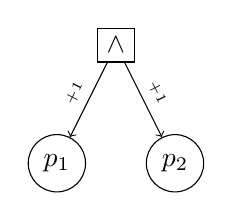
\begin{tikzpicture}[baseline=(root.base)]
          \node (root) [draw, black, rectangle] {$\land$} 
            child { node [draw, black, circle] {$p_1$}
            edge from parent [->]
            node[above, sloped, font=\tiny] {+1} }
            child { node [draw, black, circle] {$p_2$}
            edge from parent [->]
            node[above, sloped, font=\tiny] {+1} };
        \end{tikzpicture}
        \hspace{25pt}
        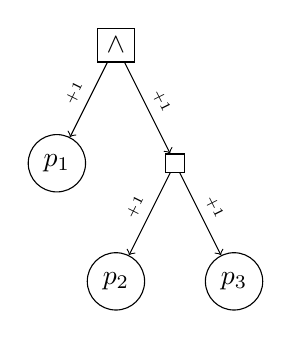
\begin{tikzpicture}[baseline=(root.base)]
          \node (root) [draw, black, rectangle] {$\land$} 
            child { node [draw, black, circle] {$p_1$}
            edge from parent [->]
            node[above, sloped, font=\tiny] {+1} }
            child { node [draw, black, rectangle] {$\Un$}
                child { node [draw, black, circle] {$p_2$}
                edge from parent [->]
                node[above, sloped, font=\tiny] {+1} }
                child { node [draw, black, circle] {$p_3$}
                edge from parent [->]
                node[above, sloped, font=\tiny] {+1} }
            edge from parent [->]
            node[above, sloped, font=\tiny] {+1} 
            };
        \end{tikzpicture}
        \label{fig:formula_ast}
    \end{figure}

    We represent LTL formulae as abstract syntax trees (ASTs) using a typed class hierarchy rooted at a \texttt{Formula} base class. Each node in the tree is an instance of one of nine subclasses: \texttt{Atom} for atomic propositions $p_0, p_1, \ldots$; four unary operator classes \texttt{Not} $(\neg)$, \texttt{Next} $(X)$, \texttt{Eventually} $(F)$, and \texttt{Globally} $(G)$, each wrapping a single child \texttt{Formula}; and four binary operator classes \texttt{And} $(\land)$, \texttt{Or} $(\lor)$, \texttt{Implies} $(\to)$, and \texttt{Until} $(\Un)$, each wrapping a left and right child \texttt{Formula}. Formulae are built by recursive composition: any \texttt{Formula} instance may serve as the child of any operator node, producing trees of arbitrary nesting depth. Two examples are shown in Figure~\ref{fig:formula_ast}.

    Every subclass implements a \texttt{\_\_str\_\_} method that produces a fully parenthesised, prefix-notation string. Atoms are rendered as \texttt{p\_i}, unary operators as \texttt{(OP child)}, and binary operators as \texttt{(left OP right)}. This string is  \emph{canonical}, in the sense that there is an injective mapping from formulae to strings, and is used for syntactic deduplication and as the input sequence consumed by the tokenizer.

    Two further properties are central to dataset construction. First, the \emph{depth} of a formula is defined recursively: an atom has depth $0$, and any operator node has depth $1 + \max(\text{child depths})$. This is illustrated in Figure~\ref{fig:formula_ast}: the left tree has depth $1$ and the right tree has depth $2$, as indicated by the $+1$ label on each edge. Depth is the primary measure of formula complexity and will be used in the sampler described in the following section to bound the complexity of the generated formulae. Second, \emph{syntactic equality} is defined as recursive node-wise comparison: two formulae are equal if and only if they are the same operator class with equal children at every position in the tree. By injectivity of the \texttt{\_\_str\_\_} function, we may also take syntactic equality between two formulae as the string equality of their respective \texttt{\_\_str\_\_} representations.
    
    \section{Formula Sampling and Dataset Generation}

    We generate LTL formulae by sampling ASTs using a procedure parameterized by \texttt{p\_leaf\_range}, \texttt{max\_depth}, \texttt{n\_ap}, and a \texttt{force\_tree} flag. At each node, a leaf probability $p_{leaf}$ is drawn uniformly from \texttt{p\_leaf\_range}. With probability $p_{leaf}$, the node is instantiated as an \texttt{Atom}, selecting a proposition $p_i$ uniformly at random from $\{p_0, \ldots, p_{n_{ap}-1}\}$. Otherwise, an operator is drawn uniformly from $\{\neg, \X, \F, \G, \land, \lor, \to, \Un \}$. Once the recursion reaches \texttt{max\_depth}, a leaf is forced regardless of the drawn probability. The \texttt{force\_tree} flag prevents the root from being instantiated as a bare atom, ensuring every sampled formula contains at least one operator.

    \begin{algorithm}
        \caption{Recursive formula sampler. The outer call is $\texttt{Gen}(0,\, p_{leaf},\, \texttt{force\_tree})$ with $p_{leaf} \sim \mathrm{Uniform}[\texttt{p\_min}, \texttt{p\_max}]$. Redundant nesting denotes the combinations $\G(\G\,\phi)$, $\F(\F\,\phi)$, and $\neg\neg\phi$.}
        \label{alg:formula_sampling_algorithm}
        \begin{algorithmic}[1]
        \Require $\texttt{n\_ap}$,\ $[\texttt{p\_min}, \texttt{p\_max}]$,\ $\texttt{max\_depth}$,\ $\texttt{force\_tree}$
        \Function{Gen}{$d$,\ $p_{leaf}$,\ $force\_op$}
            \If{$d \geq \texttt{max\_depth}$}
                \State \Return $\texttt{Atom}(p_i)$,\quad $i \sim \mathrm{Uniform}\{0,\ldots,n_{ap}-1\}$
            \EndIf
            \If{\textbf{not} $force\_op$ \textbf{and} $\mathrm{Uniform}(0,1) < p_{leaf}$}
                \State \Return $\texttt{Atom}(p_i)$,\quad $i \sim \mathrm{Uniform}\{0,\ldots,n_{ap}-1\}$
            \EndIf
            \State $\texttt{op} \sim \mathrm{Uniform}\{\neg,\, \X,\, \F,\, \G,\, \land,\, \lor,\, \to,\, \Un\}$
            \If{$\texttt{op} \in \{\neg,\, \X,\, \F,\, \G\}$}
                \Repeat
                    \State $\texttt{child} \leftarrow \texttt{Gen}(d+1,\, p_{leaf},\, False)$
                \Until{$\texttt{op}(\texttt{child})$ is not redundantly nested}
                \State \Return $\texttt{op}(\texttt{child})$
            \Else
                \State $p_l,\, p_r \sim \mathrm{Uniform}[\texttt{p\_min}, \texttt{p\_max}]$
                \State $\texttt{left} \leftarrow \texttt{Gen}(d+1,\, p_l,\, False)$
                \Repeat
                    \State $\texttt{right} \leftarrow \texttt{Gen}(d+1,\, p_r,\, False)$
                \Until{$\texttt{right} \neq \texttt{left}$}
                \State \Return $\texttt{op}(\texttt{left},\, \texttt{right})$
            \EndIf
        \EndFunction
        \end{algorithmic}
    \end{algorithm}

    
    Two structural constraints are enforced by rejection during sampling, as shown in Algorithm~\ref{alg:formula_sampling_algorithm}. First, redundant unary nesting is avoided: the combinations $\G(\G\,\phi)$, $\F(\F\,\phi)$, and $\neg\neg\phi$ are resampled whenever they arise, as they introduce syntactic redundancy without adding semantic content. Second, the two children of any binary operator must be syntactically distinct; if the left and right subtrees are equal under structural equality, the right child is resampled. Together these constraints reduce the proportion of trivially redundant formulae in the generated data without imposing any constraint on formula semantics.
    
    The sampled formulae are stored a dataset consisting of pairs of formulae and their respective semantic embedding (for details about the semantic embedding of formulae, see Chapter~\ref{chap:kernel}). Each item in the dataset yields the formula AST, its $M$-dimensional embedding vector, and a dataset index, together with the formula's canonical string and satisfaction vector when these are requested at construction time. The embedding is computed once at dataset construction and stored alongside the formula, rather than being recomputed at training time.

    \section{Tokenization}
    The \texttt{LTLTokenizer} maps a formula AST to a sequence of integer token IDs. The vocabulary is composed of three groups: four special tokens (\texttt{<pad>}, \texttt{<bos>}, \texttt{<eos>}, \texttt{<unk>}), eight operator tokens (\texttt{\textasciitilde}, \texttt{AND}, \texttt{OR}, \texttt{->}, \texttt{X}, \texttt{F}, \texttt{G}, \texttt{U}), two parentheses tokens (\texttt{(}, \texttt{)}) and $n_{ap}$ proposition tokens (\texttt{p\_0}, \ldots, \texttt{p\_{n-1}}). The total vocabulary size is $14 + n_{ap}$.
    
    Encoding proceeds in two steps. The formula's canonical string produced by \texttt{\_\_str\_\_} as described in Section~\ref{sec:formula_representation} is first split into tokens by greedy left-to-right matching against the vocabulary. The token sequence is then wrapped with \texttt{<bos>} and \texttt{<eos>} boundary markers and mapped to integer IDs. A batch of these encoded sequences, each paired with the corresponding formula's semantic embedding, forms the complete input to \texttt{LTLModel}: the token IDs as \texttt{input\_ids} and the embeddings as the \texttt{Semantic Embedding Hidden States}.

    \section{Model Architecture}
    \texttt{LTLModel} is our custom model class, built on \textit{HuggingFace}'s \texttt{GPT2LMHeadModel} with cross-attention enabled, through which all forward-pass and generation calls are routed. \texttt{GPT2LMHeadModel} couples a standard GPT-2 transformer backbone with a linear LM Head, which projects each hidden state to a logit vector over the vocabulary at every decoding step (see the \textit{HuggingFace} \href{https://github.com/huggingface/transformers/blob/v4.57.0/src/transformers/models/gpt2/modeling_gpt2.py#L981}{source} for implementation details). The full architecture is illustrated in Figure~\ref{fig:ltl_model_architecture}.

    \begin{figure}[ht]
    \centering
    \caption{Architecture diagram of GPT2LMHeadModel with cross attention enabled.}
    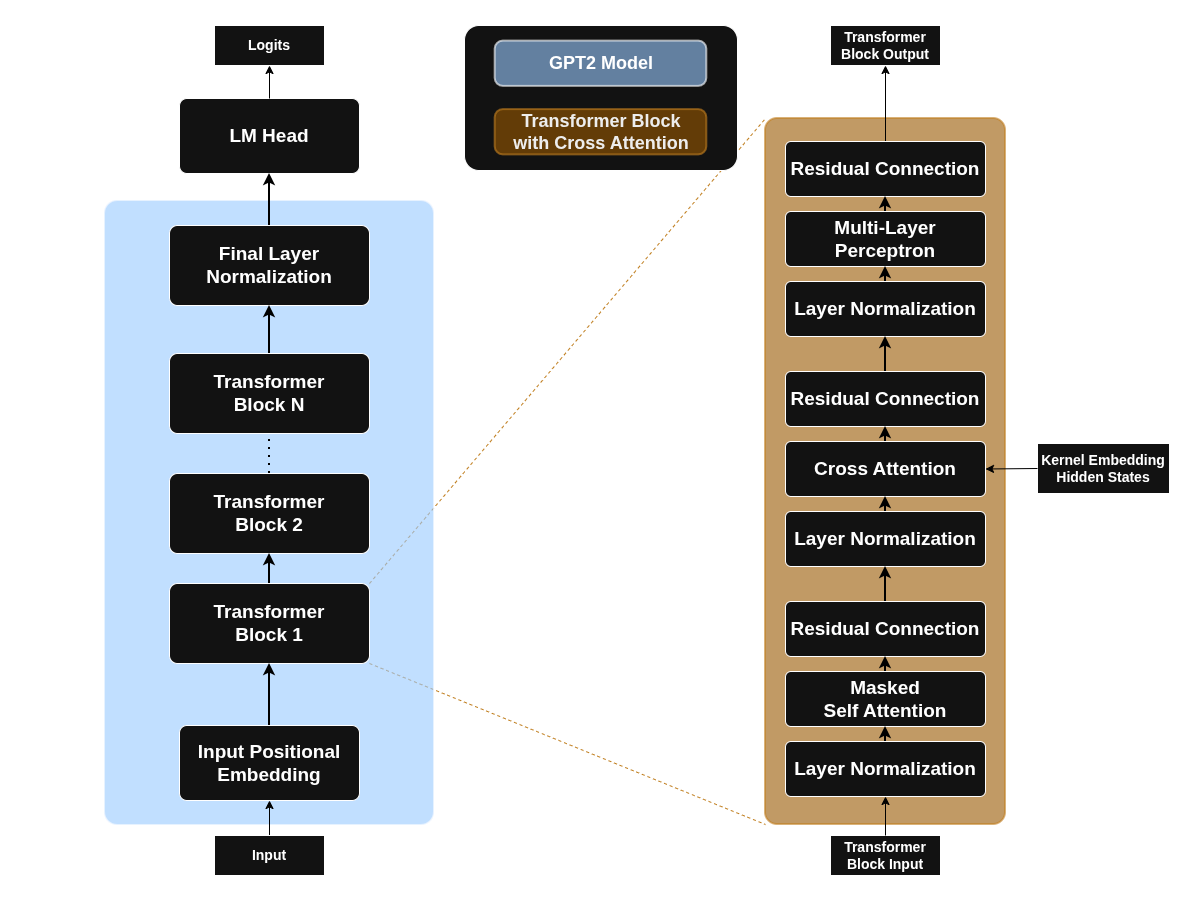
\includegraphics[width=1\linewidth]{Figures/LTLModel_Architecture.png}
    \label{fig:ltl_model_architecture}
    \end{figure}
    
    The single departure from the standard GPT-2 architecture is the insertion of a Cross Attention block within each Transformer Block. In the vanilla configuration, each Transformer Block applies a Layer Normalization followed by Masked Self Attention and a Residual Connection, then a second Layer Normalization followed by a Multi-Layer Perceptron and a final Residual Connection. Enabling cross-attention inserts a third sublayer between the first Residual Connection and the MLP: a Layer Normalization, Cross Attention, and Residual Connection. This Cross Attention block allows the decoder's hidden states to use the \emph{Semantic Embedding Hidden States} $\bm{E}_{sem} \in \mathbb{R}^M$ (a fixed vector summarizing the target formula's satisfaction behavior over a sample of traces, see Chapter~\ref{chap:kernel}), as an external conditioning signal. Rather than supplying the conditioning signal once at the input as a prefix, this mechanism makes it available to the decoder at every layer and at every decoding step.
    
    The Cross Attention block operates as follows. Let $\bm{h}_t \in \mathbb{R}^d$ denote the decoder hidden state at position $t$ after the Layer Normalization following the first Residual Connection. The \emph{Query}, \emph{Key}, and \emph{Value} vectors are produced by three separate learned projections:
    \begin{align}
        \bm{Q}_t     &= \bm{W}^{cross}_q \bm{h}_t       & \in \mathbb{R}^{d_k}\\
        \bm{K}_{sem} &= \bm{W}^{cross}_k \bm{E}_{sem}   & \in \mathbb{R}^{d_k}\\
        \bm{V}_{sem} &= \bm{W}^{cross}_v \bm{E}_{sem}   & \in \mathbb{R}^{d_k}
    \end{align}
    where $\bm{W}^{cross}_q \in \mathbb{R}^{d_k \times d}$ maps the decoder state to a query, and $\bm{W}^{cross}_k, \bm{W}^{cross}_v \in \mathbb{R}^{d_k \times M}$ project the Semantic Embedding Hidden States into a key and a value. The cross-attention output at position $t$ is $a_t\,\bm{V}_{sem}$, where the scalar attention weight $a_t \in \mathbb{R}$ is computed from the dot product $\bm{Q}_t \cdot \bm{K}_{sem} \in \mathbb{R}$:
    \begin{equation}
        a_t = \mathrm{softmax}\!\left(\frac{\bm{Q}_t \cdot \bm{K}_{sem}}{\sqrt{d_k}}\right)
    \end{equation}
    \noindent Since $\bm{E}_{sem}$ is presented as a single conditioning token, the softmax is taken over this one score and evaluates trivially to $a_t = 1$. The cross-attention output therefore reduces to $\bm{V}_{sem} \in \mathbb{R}^{d_k}$ at every position $t$, which is projected back to $\mathbb{R}^d$ and added to $\bm{h}_t$ through the Residual Connection. Within each Transformer Block, every decoder position $t$ receives the same additive update $\bm{V}{sem}$. The stregth of this update is governed entirely by the magnitude of $\bm{V}_{sem}$, which is bounded by $\Vert\bm{W}^{cross}_v\Vert\,\Vert\bm{E}_{sem}\Vert$. We return to the implications of this property in Section~\ref{sec:the_embedding_kernel}, where it motivates our choice of the covariance measure over other, normalized, alternatives.
    

\chapter{The Linear Temporal Logic Kernel and Formula Embedding} \label{chap:kernel}
    In section \ref{sec:kernel_methods} we introduced the concept of a kernelized representation of logical formulae, directly based in the semantics of the logic. In order to condition a  generator of LTL formulae on the desired temporal behavior that we want the generated formula to display, we have to be able to provide the machine with a \emph{fixed}, \emph{finite}, and \emph{syntax-invariant} representation of that formula's semantics. In this chapter we will be formalizing the \textit{Linear Temporal Logic Kernel} and the respective semantic embedding of a formula $\phi$ that we produce with it.

    \section{Constructing the Semantic Embeddings}
    Semantically, a formula $\phi$ can be characterized, up to semantic equivalence, by a satisfaction vector $\chi_\phi \in \{0,1\}^\Sigma$, where the $i$'th element of the vector indicates the formula's satisfaction on the associated trace $\sigma^i \in \Sigma$:
    \begin{equation}
        \chi_\phi^i = 1 \iff \sigma^i \vDash \phi
    \end{equation}
    A representation of this kind would serve as the ideal candidate considering our requirement of being syntax-invariant. However, it is also infeasible to compute. Even after making the move from infinite trace semantics to a finite trace semantics, the size of a vector of this kind would be enormous --- $2^{100}$ for interpretations over $T=20$ timesteps with $5$ atomic propositions. Thus, the two other requirements on our representation of being \emph{fixed} and (feasibly) \emph{finite} lead us to construct two further reductions that will finally allow us to use the formula's semantics as a conditioning signal for sequence generation.

    The first of the two reductions deals with the computationally infeasible size of the trace space directly. In order to make the representation of the satisfaction vector feasible, we sample a subset of size $N$ of the total trace space and restrict $\chi_\phi$ to it to obtain its approximation $\satvec_\phi$. With $N$ now being a hyperparameter that is under our control, we must pick it carefully such that it is large enough to obtain an approximation $\satvec_\phi$ that is useful and not too prone to errors, while being small enough to work with in practice.

    The second reduction brings this sampled satisfaction vector $\satvec_\phi$ down from $\mathbb{R}^N$ to a lower-dimensional summary in $\mathbb{R}^M$, with $M \ll N$. The natural way to construct such a reduction is to compare $\satvec_\phi$, in some fashion, against a fixed set of $M$ reference vectors $\{r_1, \dots, r_M\} \subset \mathbb{R}^N$, with each coordinate of the embedding recording how $\satvec_\phi$ relates to one of these references. The embedding as a whole is then a \emph{profile of relationships}, and its construction is determined by two important design choices: $1)$ what the reference vectors should be, and $2)$ how the comparison between $\satvec_\phi$ and each reference is computed. We address the first in the remainder of this section and the second is the subject of \S\ref{sec:the_embedding_kernel}.

    Two natural candidates suggest themselves from the dimensionality reduction literature. The first and simplest is a random projection, with entries drawn i.i.d.\ from a normal distribution. By the Johnson--Lindenstrauss lemma ~\cite{johnson_extensions_1984,dasgupta_elementary_2003} such a projection preserves pairwise distances in $\satvec$-space, up to a factor of $1\pm \epsilon$ for $\epsilon \in (0,1)$. Irrespective of whether such a projection would be able to preserve enough of the metric geometry of the $\satvec$ space for the amount of training data that we need, the main reason to reject this approach is because it loses the domain-based interpretation that makes traditional symbolic regression so desirable. With this solution every coordinate in the embedding vector is is a random linear combination of $\satvec_\phi$'s satisfaction entries, which seizes to carry any LTL-specific interpretation. A second solution is a \textit{Principal Component Analysis} (PCA) based reduction ~\citep{van_der_maaten_dimensionality_2007, hasan_review_2021}, in which the reference vectors $\{r_i\}$ are taken to be the top-$M$ variance-explaining directions of a satisfaction matrix built from a set of reference formulae (i.e.\ PCA on $\satvec$-vectors). Each coordinate of the embedding is then $\satvec_\phi$'s projection onto a direction of maximal explained variance in the reference set. Again, the resulting embedding coordinates do not lend themselves to any interpretation that is directly available from the context of LTL. For our application we will want to use a reduction that maintains this natural semantic interpretation.

    Instead, we opt for a more directly interpretable reduction and choose our reference vectors to be the satisfaction vectors of a set of \emph{anchor formulae} $\Psi = {\psi_1, \dots, \psi_M}$, with the $i$-th row equal to $\satvec_{\psi_i}$. The embedding then takes the form 
    \begin{equation}
        \emb(\phi)_i = \langle\satvec_\phi, \satvec_{\psi_i}\rangle
    \end{equation}
    i.e.\ a vector of similarities between $\phi$'s satisfaction vector and each anchor's. This choice has some desirable properties that the alternatives lack. 
    
    First, every coordinate is \emph{named}: $\emb(\phi)_i$ records the relationship between $\phi$ and a specific LTL formula $\psi_i$, which can be written down, inspected, and reasoned about by an human reader. 
    
    Second, this named structure is also meaningful to the model. Aligning the representation of the conditioning signal with the structure of the generator's output language is a form of relational inductive bias \citep{battaglia_relational_2018}: each conditioning dimension corresponds to the similarity of the target formula to an entity in the model's output language. Therefore, the decoder's prior knowledge of LTL should, in principle, transfer to its interpretation of the conditioning signal. This aligns with a broader argument in compositional-generalization research that neural sequence models benefit from being equipped with explicit, named structural components that the network can reference compositionally, rather than being expected to discover compositional structure implicitly from training data alone \citep{lake_building_2017, lake_generalization_2018}. Lake and Baroni \citep{lake_generalization_2018} specifically argue for "manually-encoded or (ideally) learned functions" for interpreting the individual building blocks of the input language. Our anchor-based conditioning is related to this idea but adopts it in a static and comparative (rather than operational) way, supplying the model with a fixed library of LTL probes, accessible via cross-attention, against which the target formula is evaluated. 
    
    The rest of this chapter will be devoted to making this embedding precise. Firstly, we will make concrete our choice for the similarity measure that sets up the semantic embedding and discuss the properties that make it desirable for use in training our transformer model. Then, we will lay out the procedure used to select the specific anchor set $\Psi$. Lastly, we will consider our method for sampling the set of traces against which the satisfaction vectors $\satvec$ are produced, reviewing the statistical power that comes with a sample size of $N$.

    \section{The Embedding Kernel}\label{sec:the_embedding_kernel}
    Thus far in this chapter we have been explicitly avoiding the use of the term \emph{kernel} to characterize the similarity measure between $\phi$ and the anchors. Plainly speaking, any real vector space equipped with an inner product $\langle \cdot, \cdot \rangle$ (together comprising the Hilbert space $\mathcal{H}$) will naturally induce a kernel by virtue of \emph{positive semi-definiteness}: for any finite collection of vectors in $\mathcal{H}$, the matrix of pairwise inner products is symmetric and PSD. By translating the satisfaction behavior of a formula into this space via a feature map $f$ derived from its satisfaction vector $\satvec_\phi$, we obtain a real-valued function on pairs of formulae:
    \begin{equation} \label{eq:kernel_general_form}
        k(\phi, \psi) = \bigl\langle f(\phi), f(\psi)\bigr\rangle_\mathcal{H}
    \end{equation}
    which is symmetric and positive semi-definite on any finite formula set, with the trace sample acting as the empirical probability space over which similarity is measured. The semantic embedding introduced in the previous section is then nothing other than the partial evaluation of this kernel against the anchor set: $\emb(\phi)_i = k(\phi, \psi_i)$, an $M$-dimensional vector of kernel similarities to a fixed set of LTL formulae. The remainder of this section is concerned with evaluating four possible ways to instantiate $k$. We will first explore the intuitive properties we desire from any such instantiation, before returning to Equation~\ref{eq:kernel_general_form} at the end of this section to prove their validity as a kernel. We will refer to our final choice as the \emph{Linear Temporal Logic Kernel}.
    
    Before we start we have some obligations that we should not try to escape from. The term \emph{kernel} carries a lot of mathematical weight of which we do not make full use in the present work. Nonetheless, we believe it is beneficial to have this discussion in the light of kernel methods for Linear Temporal Logic, as a lot of the recent literature in the field from which this project borrows has shifted in this direction ~\citep{bortolussi_kernel_2020,bortolussi_learning_2022,candussio_bridging_2025,saveri_stl2vec_2024}. Kernel methods have a wide range of applications in the field of LTL specification mining, beyond their use in the construction of the semantic embedding put forward in this chapter, and a formal definition for LTL kernels has not yet been given. Doing this opens up possible future research avenues, which we will discuss in section ~\ref{sec:future_work}. Therefore, running the risk of overstepping its proper scope, we will adopt the kernel terminology with the necessary demarcation of which of its properties are relevant to the construction of our datasets and training of our model. 

    With this preamble out of the way, it is time to formalize the inner product we adopt in constructing the semantic embedding $\emb(\phi)$. Four possible kernel functions were considered: $k^{\cdot}$ the kernel with dot-product on binary satisfaction vectors, $k^{\cos}$ the kernel with cosine similarity on binary satisfaction vectors, $k^{\pm}$ the kernel with dot-product on signed satisfaction vectors (with $False$ mapped to $-1$, and $True$ mapped to $1$), and lastly $k^{\cov}$ the kernel with covariance on binary satisfaction vectors.  The justification for choosing the last of these four is best understood when we consider how the other options fail to properly encode the kind of relation we want between $\phi$ and the anchors. In what follows we will be setting up and arguing for two things simultaneously: Firstly, what we would \emph{intuitively} want our kernel value to represent, and then secondly, what inner product most faithfully fulfills this intuition.

    \subsection{Dot Product Kernel}
    We start with the dot product on the binary satisfaction. For two satisfaction vectors $\satvec_\phi$ and $\satvec_\psi$, the dot product similarity is defined as follows:
    \begin{equation}
        k^{\cdot}(\phi,\psi):=\satvec_\phi \cdot \satvec_\psi = \sum^N_{i=1} \widehat \chi^i_{\phi} \widehat \chi^i_{\psi}
    \end{equation}
    Under this choice, $\emb(\phi)$ is simply the projection through the stacked $\satvec_{\psi_i}$ satisfaction vectors. This kernel suffers fromWe should consider the case where the two formulae are each other's negations, that is $\psi \equiv \neg\phi$. In this case we would find that $k(\phi,\psi)=0$ since, by definition, their truth sets do not overlap. The problem here is not just that $k$ assigns a formula and its negation a low value, it is that $k$ conflates the very distinct negation relation (given $\neg \phi$, the satisfaction behavior of $\phi$ is determined fully) with the lack of any such relation. Ideally we want orthogonality in this space to be representative of \emph{unrelatedness} and not just \emph{mutual exclusivity}, of which negation is the most striking case. Moreover, intuition decrees that the negation case should be mapped to the minimum kernel value, as it signifies maximum dissimilarity. This kernel does neither.
    
    This alone is enough to reject this measure as unfit, but there is a second failure mode that appears at the opposite end of the kernel's range that is worth highlighting: the dot product over binary satisfaction vectors cannot distinguish \emph{logical equivalence} from \emph{logical implication}. Ideally we would want our maximal values for $k(\phi,\cdot)$ to be occupied by formulae in the input domain that are logically equivalent to $\phi$, i.e. the formulae with the highest similarity scores to $\phi$ are those that are most similar in satisfaction. However, for the dot-product similarity it is the case that whenever the truthset of $\phi$ is a subset of the truthset of $\psi$, then the kernel value $k(\phi, \psi)$ will be maximal (namely the cardinality of the truthset of $\phi$). Thus for this metric it holds that maximum kernel values are attained for any formula $\psi$ that is logically implied by $\phi$.

    \subsection{Cosine Kernel}
    The second of the kernel functions, the cosine similarity between the binary satisfaction vectors, is defined as follows:
    \begin{equation}
        k^{\cos}(\phi,\psi):= \frac{\satvec_\phi \cdot \satvec_\psi}{\Vert \satvec_\phi \Vert \mkern6mu \Vert \satvec_\psi \Vert} = \frac{\sum^N_{i=1} \widehat \chi^i_{\phi} \widehat \chi^i_{\psi}}{\sqrt{\sum^N_{i=1} (\widehat \chi^i_{\phi})^2} \mkern6mu \sqrt{\sum^N_{i=1} (\widehat \chi^i_{\psi})^2}},
    \end{equation}
    representing the dot product between the satisfaction vectors normalized by the product of their respective Euclidean norms. This solution fixes the indistinguishability issue at the maximal values that the dot product kernel suffered from: $k^{\cos}(\phi,\psi) = 1$ only when the numerator $\satvec_\phi \cdot \satvec_\psi$ is exactly equal to the denominator $\Vert \satvec_\phi \Vert \mkern6mu \Vert \satvec_\psi \Vert$. This only happens exactly when the truth sets of the two formulae are the exact same. Specifically, suppose they have cardinality $S$, then the kernel value gets evaluated to $k^{\cos}(\phi,\psi) = \frac{S}{\sqrt{S} \sqrt{S}} = 1$. In the case where the truthset of $\psi$ (properly) extends the truthset of $\phi$, we no longer find that the kernel similarity between $\phi$ and $\psi$ is also maximal. Now instead, for this case, the kernel value is smaller. Let the cardinality of truthset of $\phi$ be $S$, amd that of $\psi$'s be $S^\prime$ with $S^\prime > S$. Then: $k^{\cos}(\phi,\psi) = \frac{S}{\sqrt{S} \sqrt{S^\prime}} < 1$. 

    Unfortunately, the cosine similarity based kernel does not solve the issues at the other extreme. This kernel still maps a formula and its negation to $0$, since the dot product is still the sole part of the numerator. We must look elsewhere for a solution to this problem.

    \subsection{Signed Dot Product Kernel}
    The attentive reader may have already noted that there is a glaring flaw that the previous two kernels share. What they both count is how often two formulae $\phi$ and $\psi$ are \emph{simultaneously true} on the set of traces. What neither of these metrics account for, however, is how often both formulae are also \emph{simultaneously false}. It seems intuitive that a good similarity metric should be looking for agreement on traces in both directions. One natural revision is to re-encode the satisfaction vectors from ${0,1} \to {-1,+1}$ via the map $\widehat\chi \mapsto 2\widehat\chi - \mathbf{1}$, where $\mathbf{1}$ denotes the all-ones vector in $\mathbb{R}^N$. The signed kernel then takes the form:
    \begin{equation}
        k^\pm(\phi, \psi) := (2\satvec_\phi - \mathbf{1}) \cdot (2\satvec_\psi - \mathbf{1}) = \sum^N_{i=1} (2 \widehat \chi^i_{\phi} - 1) (2 \widehat \chi^i_{\psi} - 1)
    \end{equation}
    This kernel solves both problems that disqualified the two previous ones. On the one hand, mutual exclusivity no longer gets mapped to $0$. Two mutually exclusive formulae (ones whose truthsets have an empty intersection) now receive a kernel value that depends on the size of their negated overlap. More importantly, negation is explicitly handled: when $\psi \equiv \neg\phi$, their signed satisfaction vectors point in strictly opposite directions, yielding the global minimum $k^\pm(\phi, \neg\phi) = -N$. On the other the maximum similarity is still reserved for logically equivalent formulae $\phi \equiv \psi$. Since the map we defined earlier changes only on the satisfaction vectors, we know that post transformation $\phi$ and $\psi$ still get mapped to the same point, that is $\satvec_\phi = \satvec_\psi$, so their kernel value will be $N$. Additionally, since the kernel now properly accounts disagreements in falsityset, the case where one formula logically implies the other no longer receives maximum kernel value. Disagreement on a trace now results in a negative term in the sum, properly penalizing this disagreement towards similarity. 

    At the extremes of its range, then, $k^\pm$ behaves as intuition dictates: equivalence at the maximum, negation at the minimum. What remains to be examined is the intermediate region of the kernel's range, and in particular the value $0$. We have, twice now, gestured at this region informally as the natural home for \emph{unrelated} formulae. Before asking whether $k^\pm$ places unrelated formulae here, we must make explicit precisely what we mean by "unrelatedness".
    
    We make the informal idea of \emph{unrelatedness} precise by identifying it with \emph{semantic independence}. We say that two formulae $\phi, \psi$ are \emph{semantically independent}, with respect to a probability distribution $\mathcal{T}$ over the full trace space $\Sigma$, if their satisfaction values $\chi^\sigma_\phi$ and $\chi^\sigma_\psi$, viewed as Bernoulli random variables under $\sigma \sim \mathcal{T}$, are statistically independent: for all $a, b \in \{0, 1\}$,
    \begin{equation}
        \Pr_{\sigma \sim \mathcal{T}}[\chi^\sigma_\phi = a,\, \chi^\sigma_\psi = b]
        \;=\;
        \Pr_{\sigma \sim \mathcal{T}}[\chi^\sigma_\phi = a]\,
        \Pr_{\sigma \sim \mathcal{T}}[\chi^\sigma_\psi = b],
    \end{equation}
    or equivalently $\cov_{\mathcal{T}}(\chi_\phi, \chi_\psi) = 0$.
    
    A full philosophical analysis of what semantic independence should entail for LTL is beyond the scope of the present work, but one thing that jumps out from textbook discussions of LTL is that the relativity to a distribution is an important component of any definition, and we therefore treat it as a feature rather than a defect. Linear-time temporal logic is often introduced as a formal \emph{specification language} for reactive systems ~\citep{baier_principles_2008}: a formula expresses a property that a system $S$ is said to satisfy when every trace of $S$ satisfies it. The trace ensemble against which an LTL formula is interpreted is therefore not a universal object but is bound to the system under consideration. The probabilistic setting we adopt here is a natural lift of this picture: in place of the deterministic trace set of a fixed system, we work with a probability distribution $\mathcal{T}$ over traces, which plays the same role of defining the population of behaviors against which a formula's satisfaction profile is read. The kernel embeds formula behavior under a trace distribution, so "unrelated" is naturally a statement about behavior under that same distribution. We will further discuss this topic in section \ref{sec:trace_sampling_details}. 
    
    With unrelatedness now formalized as semantic independence under $\mathcal{T}$, we can ask whether $k^\pm$ places semantically independent pairs near $0$. It does not, and the reason becomes visible once we compute the expected kernel value $\mathbb{E}\!\left[k^\pm(\phi, \psi)\right]$ for an arbitrary semantically independent pair of formulae $\phi$ and $\psi$. Writing
    \begin{equation}
    p_\phi := \Pr_{\sigma \sim \mathcal{T}}[\widehat\chi^\sigma_\phi = 1] = \mathbb{E}_{\sigma \sim \mathcal{T}}[\widehat\chi^\sigma_\phi]
    \end{equation}
    for the base rate of $\phi$ under $\mathcal{T}$ (and analogously $p_\psi$ for $\psi$), linearity of expectation reduces the kernel's sum to $N$ copies of a single per-trace term,
    \begin{equation}
        \mathbb{E}\!\left[k^\pm(\phi, \psi)\right]
        \;=\;
        N \cdot \mathbb{E}_{\sigma \sim \mathcal{T}}\!\left[(2\widehat\chi^\sigma_\phi - 1)(2\widehat\chi^\sigma_\psi - 1)\right],
    \end{equation}
    and expanding the product inside the expectation yields
    \begin{equation}
        \mathbb{E}\!\left[k^\pm(\phi, \psi)\right]
        \;=\;
        N \cdot \left(4\,\mathbb{E}_{\sigma \sim \mathcal{T}}\!\left[\widehat\chi^\sigma_\phi\, \widehat\chi^\sigma_\psi\right] - 2\,p_\phi - 2\,p_\psi + 1\right).
    \end{equation}
    The remaining joint expectation can be decomposed into a base-rate contribution and a covariance contribution via the identity $\mathbb{E}_{\sigma \sim \mathcal{T}}[\widehat\chi^\sigma_\phi\, \widehat\chi^\sigma_\psi] = p_\phi\, p_\psi + \cov_{\mathcal{T}}(\widehat\chi_\phi, \widehat\chi_\psi)$. Substituting and grouping the resulting terms gives the general expression
    \begin{equation}\label{eq:kpm_general}
        \mathbb{E}\!\left[k^\pm(\phi, \psi)\right]
        \;=\;
        N \cdot \Bigl(
            \underbrace{(2\,p_\phi - 1)(2\,p_\psi - 1)}_{\text{marginal product}}
            \;+\;
            \underbrace{4\,\cov_{\mathcal{T}}(\widehat\chi_\phi, \widehat\chi_\psi)}_{\text{covariance contribution}}
        \Bigr),
    \end{equation}
    which holds for any pair of formulae, independent or not. Semantic independence under $\mathcal{T}$ means that $\cov_{\mathcal{T}}(\widehat\chi_\phi, \widehat\chi_\psi) = 0$, in which case equation~\eqref{eq:kpm_general} reduces to
    \begin{equation}\label{eq:kpm_indep}
        \mathbb{E}\!\left[k^\pm(\phi, \psi)\right]
        \;=\;
        N \cdot (2\,p_\phi - 1)(2\,p_\psi - 1),
    \end{equation}
    which ranges over the entire kernel scale $[-N, N]$ as the base rates vary. Explicitly, two semantically independent formulae $\phi$ and $\psi$ each satisfied on $90\%$ of traces yield $k^\pm(\phi,\psi) \approx 0.64\,N$, heavily positive, despite the formulae being independent by construction. The same holds for two low-base-rate formulae, whose signed vectors are jointly dominated by $-1$ entries and therefore also produce a large positive value. For the asymmetric case, in which we have a high- and low-base-rate independent pair, the kernel value is strongly negative. The signed dot product kernel only maps two independent formulae to $0$ in case either $p_\phi$ or $p_\psi$ equals exactly $\tfrac{1}{2}$. Additionally, by equation~\eqref{eq:kpm_general}, the zero region of $k^\pm$ is also populated by \emph{non-independent} pairs whose covariance happens to cancel the product of their marginals. The zero region of $k^\pm$ is therefore neither necessary nor sufficient for semantic independence: it is the locus of an algebraic coincidence, not the locus of any semantic property.

    \subsection{Covariance Kernel}
    This brings us finally to the last of the kernel functions $k^{\cov}$, the covariance kernel. The decomposition of equation \eqref{eq:kpm_general} makes the natural remedy immediately apparent: to construct a similarity measure that isolates semantic independence and correctly maps it to zero, we must strip away the marginal product. We accomplish this by centering the satisfaction vectors around their respective base rates before taking their dot product. Let $\bar{\chi}_\phi = \frac{1}{N}\sum_{i=1}^N \widehat{\chi}^i_\phi$ be the empirical base rate (mean satisfaction) of $\phi$ over our sampled traces. The covariance kernel is defined as:
    \begin{equation}
        k^{\cov}(\phi, \psi) := \frac{1}{N} \sum_{i=1}^N (\widehat{\chi}^i_\phi - \bar{\chi}_\phi) (\widehat{\chi}^i_\psi - \bar{\chi}_\psi)
    \end{equation}
    By construction, this sum is exactly the empirical covariance of the two satisfaction vectors over the trace sample. As a direct consequence, the expected kernel value for any two semantically independent formulae evaluates to $0$. Crucially, for binary variables, the converse holds as well: a true covariance of $0$ strictly implies independence. While our finite sample size $N$ subjects the kernel to empirical sampling noise, the Law of Large Numbers guarantees that as $N \to \infty$, the empirical covariance asymptotically approaches this true population covariance. In the limit, therefore, orthogonality in our kernel space is both a necessary and sufficient condition for genuine semantic independence. We want to make special mention of the the subclass of \textit{tautologies} and \textit{contradictions} for which this mapping holds with respect to any formula. For tautologies and contradictions, their satisfaction vectors are the constants $\mathbf{1}$ and $\mathbf{0}$, respectively, on any sample $\widehat\Sigma$. A constant is trivially independent of any random variable, and the kernel therefore assigns them value $0$ against every formula $\psi$. We return to the role of this property in the semantic embedding $\emb(\phi)$ at the end of this section.
    
    Before continuing, we should deliver on our earlier promise to formally guarantee that the four similarity measures $k^\cdot$, $k^{\cos}$, $k^\pm$, and $k^{\cov}$ actually constitute proper kernel functions. As we alluded to at the start of this section, a symmetric bivariate function $k$ is a valid positive semi-definite (PSD) kernel if it can be expressed in the form of equation~\eqref{eq:kernel_general_form}, that is, as an inner product between elements in a Hilbert space $\mathcal{H}$ produced by a feature map $f$. Each of our four proposed functions can be formulated exactly in this way by taking $\mathcal{H}$ to be $\mathbb{R}^N$ equipped with the standard dot product, and instantiating $f$ as a specific transformation of the satisfaction vector. Specifically: for $k^\cdot$, $f(\phi) = \satvec_\phi$; for $k^{\cos}$, $f(\phi) = \frac{\satvec_\phi}{\Vert \satvec_\phi \Vert}$; for $k^\pm$, $f(\phi) = 2\satvec_\phi - \mathbf{1}$; and for $k^{\cov}$, $f(\phi) = \frac{1}{\sqrt{N}} (\satvec_\phi - \bar{\chi}_\phi \mathbf{1})$. Because they can all be written strictly as real dot products on these transformed feature vectors, their associated kernel matrices on any finite set are guaranteed to be Gram matrices.
    
    What remains is to verify that the desirable behavior of $k^\pm$ at the boundaries of its range is preserved here. As established previously, we want it to be the case that the extreme ends of the kernel value range are inhabited \emph{only} by logical equivalence and negation, and that they are not silently shared with the strictly weaker relations of \emph{logical implication} and \emph{mutual exclusivity} as we saw with the previous kernels. To this end we show that, for two formulae $\phi$ and $\psi$, the pair receives maximum kernel value if and only if they are semantically equivalent with respect to the sampled traces $\widehat \Sigma$. Similarly we show that the pair receives minimal kernel value if and only if they are each other's negation.

    We begin with the positive extreme. The sufficiency direction is immediate: when $\phi$ and $\psi$ agree on every sampled trace, $\widehat\chi^i_\psi = \widehat\chi^i_\phi$ for all $i$ and hence $\bar\chi_\psi = \bar\chi_\phi$, so each summand of $k^{\cov}$ collapses to the square $(\widehat\chi^i_\phi - \bar\chi_\phi)^2$ and the kernel evaluates to $k^{\cov}(\phi, \psi) = \operatorname{var}(\widehat\chi_\phi)$. For the necessity direction we argue by contraposition: we show that whenever $\phi$ and $\psi$ disagree on at least one trace, then $k^{\cov}(\phi, \psi)$ falls strictly below the self-paired value. Suppose then that $\phi$ and $\psi$ are not logically equivalent on $\widehat\Sigma$, meaning there exists a non-empty set of traces $D \subseteq \widehat\Sigma$ on which their evaluations differ, while they agree on the remainder $A = \widehat\Sigma \setminus D$. We can partition the kernel's sum accordingly:
    \begin{equation}
        k^{\cov}(\phi, \psi) = \frac{1}{N} \sum_{i \in A} (\widehat{\chi}^i_\phi - \bar{\chi}_\phi) (\widehat{\chi}^i_\psi - \bar{\chi}_\psi) + \frac{1}{N} \sum_{i \in D} (\widehat{\chi}^i_\phi - \bar{\chi}_\phi) (\widehat{\chi}^i_\psi - \bar{\chi}_\psi)
    \end{equation}
    For any trace $i \in D$, we have $\widehat\chi^i_\phi \neq \widehat\chi^i_\psi$. Because satisfaction values are strictly binary, one formula must evaluate to $1$ while the other evaluates to $0$. Consequently, the term inside the second sum takes one of two forms: either $(1 - \bar\chi_\phi)(0 - \bar\chi_\psi)$ or $(0 - \bar\chi_\phi)(1 - \bar\chi_\psi)$. Assuming neither formula is trivial on $\widehat\Sigma$ (i.e., their base rates $\bar\chi_\phi, \bar\chi_\psi \in (0, 1)$), both of these expressions evaluate to strictly negative values: $-(1 - \bar\chi_\phi)\bar\chi_\psi$ and $-\bar\chi_\phi(1 - \bar\chi_\psi)$, respectively. 
    
    Thus, every trace in $D$ contributes a strictly negative amount to the sum. Meanwhile, the total positive contribution from the matching traces in $A$ can be no larger than the sum over all $N$ traces in case we have perfect agreement. Because $D$ is assumed to be non-empty, its total negative contribution strictly diminishes the value of $k^{\cov}(\phi, \psi)$ below the maximum self-paired value, proving that the maximum is attained if and only if $\phi$ and $\psi$ are logically equivalent on $\widehat\Sigma$.
    
    An analogous argument applies to the negative extreme. The global minimum occurs when $\phi$ and $\psi$ are strict negations, in which case $A$ is empty and the sum consists entirely of maximal negative contributions from $D$. If the formulae are not strict negations, $A$ is non-empty, and the positive contributions from traces where $\phi$ and $\psi$ agree will ensure the kernel evaluates strictly above the global minimum.
    
    However, while the $k^{\cov}$ kernel captures each of the properties we laid out, the mean-centering operation by which we achieve this introduces a subtle but significant vulnerability into the definition of the semantic embedding $\emb(\phi)$. Because centering explicitly discards the base rate $\bar{\chi}_\phi$, the magnitude of the resulting semantic embedding is strictly governed by the formula's temporal variance. Consider the embedding vector $\emb(\phi) = [k^{\cov}(\phi, \psi_1), \dots, k^{\cov}(\phi, \psi_M)]^T$. By the Cauchy--Schwarz inequality, the magnitude of each coordinate is strictly bounded by $|k^{\cov}(\phi, \psi_i)| \leq N \operatorname{std}_\phi \operatorname{std}_{\psi_i}$, where $\operatorname{std}$ denotes the empirical standard deviation over the trace sample. If $\phi$ is a low-variance formula, then $\operatorname{std}_\phi \approx 0$, forcing every coordinate of $\emb(\phi)$ toward zero. Consequently, the embedding $\emb(\phi) \approx \mathbf{0}$ for a nearly constant formula becomes completely indistinguishable from the embedding of a highly complex, high-variance formula that simply happens to be semantically independent of every anchor $\psi_i \in \Psi$.
    
    This brings us back to case of \textit{tautologies} and \textit{contradictions} we noted earlier. Because the satisfaction vectors of both a tautology and a contradiction have standard deviation exactly zero, the covariance kernel maps them both to zero, regardless of the formula we compare them against. The resulting kernel embedding for both is the $\mathbf{0}$. At first glance this might seem like a flaw. After all, why should two formulae with directly opposing semantics have the same semantic embedding? However if we view this from the perspective of the kernel, any other mapping for $k^\cov(\top,\cdot)$ and $k^\cov(\bot,\cdot)$ would represent some spurious relation where there should in actually exist none. We want the orthogonality in our kernel space to mean precisely what we established when defining the covariance kernel above: a faithful statement of semantic independence under $\mathcal{T}$. As we have already noted, a constant random variable is independent of every other random variable by definition.
    
    This is more than a just a matter of embedding aesthetic, and the temptation to "fix" it by assigning $\top$ and $\bot$ some non-zero relationship to the anchor set runs into an immediate algebraic obstruction. The covariance kernel satisfies the bilinear identity
    \begin{equation} \label{eq:negation_identity}
        k^{\cov}(\phi, \neg\psi) \;=\; \cov_\mathcal{T}(\widehat\chi_\phi,\, 1 - \widehat\chi_\psi) \;=\; -k^{\cov}(\phi, \psi),
    \end{equation}
    which is the same identity that pinned negation to the global minimum in the boundary proof above. Suppose, then, that we wished to assign $k^{\cov}(\top, \psi) = c$ for some fixed non-zero $c$ and every formula $\psi$. Applied to a negation pair $\{\psi, \neg\psi\}$, this stipulation would require $k^{\cov}(\top, \neg\psi) = c$ by uniformity across formulae and $k^{\cov}(\top, \neg\psi) = -c$ by equation~\eqref{eq:negation_identity}, forcing $c = -c$ and therefore $c = 0$. The mapping of tautologies and contradictions to $\mathbf{0}$ is therefore not the most defensible of the available options but the only consistent one: the kernel's own algebra leaves no other fixed point. The real concern, then, is not whether $\mathbf{0}$ is the appropriate embedding for $\top$ and $\bot$, but whether this indistinguishability is a liability for our use of the kernel. We argue that it is not, and the reason has to do with the kind of questions that any solution to the problem of specification mining is designed to answer.
    
    Specification mining asks for a formula that captures a target behavioral profile: a description of which traces a system under specification should admit and which it should reject. The conditioning signal we hand to the generator is, by construction, an answer to the question \emph{which traces are we describing?}, and the embedding $\emb(\phi)$ is its representation under the kernel's geometry.
    
    Tautologies and contradictions are not specifications in this sense. The trace set admitted by $\top$ is the entirety of $\Sigma$, and the trace set admitted by $\bot$ is empty. Neither carves the trace space into a meaningful subset, neither rules anything out, and neither expresses a property a system either does or does not have in any non-trivial sense. They are formulae whose semantics make them well-defined objects of the logic, but their role in specification mining is none. Read in this light, the kernel's collapse of $\emb(\top)$ and $\emb(\bot)$ to $\mathbf{0}$ is not a failure to distinguish two formulae that ought to be distinguished, but a faithful report that the conditioning question they pose is empty.
    
    The key question that remains is whether this variance sensitivity is a boon or a liability for our downstream sequence generator. The Cauchy--Schwarz bound dictates that a formula $\phi$ with intrinsically low variance under $\mathcal{T}$ will produce tightly bounded covariance scores, resulting in a low-magnitude semantic embedding $\emb(\phi)$. The standard remedy in dimensionality reduction would be to divide out this variance by applying cosine normalization, exactly as we did for $k^{\cos}$, transforming our covariance kernel into an empirical Pearson correlation and forcing all formula embeddings onto a unit scale. But is that something we should want?

    To answer this, we must look at how the transformer model actually incorporates this conditioning signal. In our architecture, the $M$-dimensional semantic embedding is injected into the cross-attention block as a \emph{single} conditioning token. Crucially, as Kobayashi et al. ~\citep{kobayashi_attention_2020, kobayashi_incorporating_2021} established in their analysis of the transformer architecture, the functional strength of any conditioning signal injected into the generation process is governed by the vector norm of its corresponding Value vector. Inside each cross-attention block, our embedding $\emb(\phi)$ is multiplied by a learned weights matrix $W^V$ to produce the Value vector $V = W^V \emb(\phi)$. By the properties of linear transformations, the norm of this result is mathematically bounded by the magnitude of the input: $\Vert V \Vert \leq \Vert W^V \Vert \, \Vert \emb(\phi) \Vert$. The core intensity of the downstream conditioning signal is therefore structurally tethered to the unnormalized magnitude of the semantic embedding itself.
    
    Viewed through this lens, the variance sensitivity is a significant boon. By preserving the formula's variance rather than normalizing it away, the covariance kernel is afforded a the degree of freedom that it may learn to exploit. When the model encounters a small magnitude embedding, we want it to interpret this as: \textit{the anchors' behavioral patterns are relatively uninformative for explaining that of the target formula}. If we were to cosine-normalize the kernel, we would rob the architecture of its only mechanism to respond appropriately to the differing informativeness of the formulae's behavioral signals.

    We should be mindful, however, that a small-magnitude embedding can arise from two distinct causes. The first, and the one we have been discussing, is that $\phi$ genuinely has low variance under $\mathcal{T}$: the formula holds on almost all traces or almost none, and the faint conditioning signal this produces is precisely the response that preserving the embedding's magnitude is there to afford. The second is more troubling. The formula $\phi$ may have high variance under $\mathcal{T}$ yet happen to be nearly orthogonal to every anchor in $\Psi$, so that its rich behavior goes entirely unregistered and its embedding collapses toward $\mathbf{0}$. From the magnitude of $\emb(\phi)$ alone these two cases are indistinguishable, and it is tempting to read this as a second argument for normalization: rescaling each coordinate by $1/\operatorname{std}_\phi$ would lift the low-variance embedding to unit scale while leaving the high-variance, orthogonal one near zero, prizing the two apart and separating out the problematic cases.

    This temptation should be resisted, because the separation cuts in precisely the wrong direction. Leaving the orthogonal embedding near zero leaves the very case we would wish to repair untouched. Moreover, lifting the low-variance embedding to unit scale is not a rescue but a fabrication: those coordinates are small because the formula is very nearly constant, and amplifying them to full scale manufactures a confident profile of relationships out of sampling noise. Normalization thus \textit{corrupts} the case we mean to preserve while doing \textit{nothing} for the case we mean to fix.
    
    The orthogonality problem is therefore not one that any choice of kernel metric can resolve, since its origin does not lie in the metric at all. A high-variance formula is invisible to $\emb(\phi)$ exactly when the anchor set fails to span the directions along which that formula varies. The only genuine remedy is to ensure that our anchors cover the satisfaction space well enough so that no meaningful target formula is left orthogonal to all of $\Psi$. The problem of selecting $\Psi$ effectively is the subject of the following section.

    
    \section{Anchor Set Selection}
    Having established the embedding kernel, we now turn to the selection of the anchor set $\Psi = \{\psi_1, \dots, \psi_M\}$. To make the semantic embedding as expressive as possible, the anchors must cover a diverse and representative array of LTL behaviors, effectively spanning the space of possible trace evaluations. 
    
    While it might seem natural to select anchors that are mutually uncorrelated using the covariance kernel $k^{\cov}$, doing so discards crucial structural information. Because $k^{\cov}$ explicitly centers satisfaction vectors and strips away base rates, it is blind to absolute location in the trace space. For the purpose of providing a robust coordinate system, we want our selection metric to be sensitive to absolute truth values and spatial dispersion.
    
    If we want our anchors to be maximally dispersed across the Boolean hypercube $\{0,1\}^N$, the native measure by which to measure (dis)similarity is the Hamming distance, which counts the number of traces on which two formulae disagree. Returning to our signed dot product kernel $k^\pm$, we find it maps perfectly onto this objective. By accumulating the sum of agreements minus the sum of disagreements, $k^\pm$ acts as an exact inverse measure of Hamming distance:
    \begin{equation}
        k^\pm(\phi, \psi) = N - 2 D_H(\satvec_\phi, \satvec_\psi)
    \end{equation}
    By minimizing their pairwise $k^\pm$ similarity, we directly maximize the Hamming distance between our anchors, pushing their satisfaction vectors apart and providing broad structural coverage of the trace space.

    To make this precise, let us outline the technical details of the sampling algorithm used to construct $\Psi$. We employ a rejection-sampling scheme that enforces a strict upper bound on allowable similarity. Using the same formula sampling algorithm from \ref{alg:formula_sampling_algorithm}, the construction proceeds as follows. We set a strictly positive similarity threshold $\tau \in (0, 1)$ and initialize an empty anchor set $\Psi$. The algorithm iteratively evaluates a randomly generated candidate formula $\psi$ and computes its signed satisfaction vector $\satvec_\psi^\pm = 2\satvec_\psi - \mathbf{1}$. Because $\satvec_\psi^\pm \in \{-1, 1\}^N$, its Euclidean norm is strictly $\sqrt{N}$. We then measure the candidate's proximity to the existing ensemble by computing the normalized signed dot product against every accepted anchor $\psi_i \in \Psi$:
    \begin{equation}
        \text{sim}^\pm(\psi, \psi_i) = \frac{1}{N} k^\pm(\psi, \psi_i) = \frac{\satvec_\psi^\pm \cdot \satvec_{\psi_i}^\pm}{\Vert \satvec_\psi^\pm \Vert \; \Vert \satvec_{\psi_i}^\pm \Vert}
    \end{equation}
    If the maximum similarity score to any previously selected anchor exceeds $\tau$, the candidate formula gets rejected. If the score falls below our threshold, the candidate is appended to $\Psi$. This process iterates, resampling and rejecting as necessary, until exactly $M$ anchors have been acquired. 

    We note, however, a structural limitation in this greedy formulation. By strictly thresholding on the upper bound ($\text{sim}^\pm > \tau$), the algorithm explicitly rejects candidate formulae that are too closely aligned with existing anchors, but fails to filter on the negative extreme. Consequently, a candidate that exhibits highly \emph{negative} similarity to an existing anchor may still be accepted. While this does not violate the goal of maximizing metric dispersion directly, accepting a formula and its negation essentially commits two anchor dimensions to representing the exact same axis of the trace space. We will revisit the implications of this redundancy in Section \ref{sec:limitations}.


    \section{Trace Sampling Details} \label{sec:trace_sampling_details}
    In this section we will be discussing our sampling method for the $N$ traces that make up the trace space $\widehat \Sigma$. As discussed in section \ref{sec:the_embedding_kernel}, our measure of formula similarity is not an absolute property of the logic, but is strictly parameterized by the trace distribution $\mathcal{T}$. The formulae similarities and the resulting geometry of the semantic embeddings exist entirely with respect to $\mathcal{T}$. We will now make explicit how the target sample of $N$ traces, $\widehat\Sigma \sim \mathcal{T}$, is actually generated.

    \subsection{The Sampling Process}
    This dependency on the distribution $\mathcal{T}$ surfaces a considerable tension in the application of kernel methods to general-purpose specification mining. As we noted in Section \ref{sec:the_embedding_kernel}, LTL is conventionally evaluated against the traces of a specific reactive system. If one were mining specifications for one specific system, the true distribution $\mathcal{T}$ would be the behavioral frequencies of said system. However, we are training a general-purpose sequence model aimed at learning the mapping between generic LTL syntax and semantics. There exists no "universal" trace distribution that faithfully represents the behavior of all systems. Any choice of $\mathcal{T}$ we make is therefore fundamentally synthetic and, in the context of real-world systems, arbitrary.

    Acknowledging this does not offer us a way forward, however it leads to the realization that the aims for designing $\mathcal{T}$ should not be at mimicking any real systems but specifically at providing \emph{metric utility}. If the primary threat to our semantic embedding is orthogonality and base-rate collapse, where formulas fail to distinguish themselves from one another, then $\mathcal{T}$ must be constructed to elicit high-variance evaluations from the temporal operators, preventing them from collapsing asymptotically into trivial constants. To this end, we define our sample $\widehat\Sigma$ as a mixture of two distinct generative processes. 
    
    The first sub-population is generated via independent Bernoulli$(0.5)$ trials. At every timestep $t \in [0, T-1]$ and for every atomic proposition $p \in AP$, a truth value is drawn uniformly at random. This process yields highly entropic, chaotic trace behavior. These high-variance traces act as a robust discriminator for Boolean combinatorics and short-horizon temporal formulae, such as the $X$ operator.

    However, relying entirely on pure Bernoulli traces risks collapse for other temporal operators. Because the truth values are entirely uncorrelated across time, a globally scoped property like $G p$ becomes exponentially unlikely to be satisfied as the trace length $T$ grows, pushing its base rate toward zero. Conversely, the eventuality property $F\, p$ becomes overwhelmingly likely, pushing its base rate toward one. Under pure noise, satisfaction vectors of complex temporal formulae that rely on structural temporal patterns regress into triviality.
    
    To rescue the evaluation space from this temporal collapse, the remaining trace sample is generated via a temporally correlated Markov process. For these traces, the initial state at $t=0$ is drawn uniformly at random. For every subsequent timestep $t+1$, each atomic proposition inherits its truth value from the prior step $t$, with a small flipping probability $p_{\text{flip}}$. Additionally, we make sure that the \textit{all-true} and \textit{all-false} traces are always included in the sample. This process introduces temporal persistence into the traces. Periods of stability allow properties like $G p$ to realistically hold over significant intervals, pulling their base rates back into the informative regions of the distribution. 
    
    By blending these two generative regimes, the resulting distribution $\mathcal{T}$ ensures that our sampled trace space $\widehat \Sigma$, while not representative of any singular real-world system, provides a rigorously challenging environment. It prevents trivialization of the temporal operators and forces the semantic embedding to capture a rich, varied profile of LTL behavior.

    \subsection{Choosing $N$}
    With the trace distribution $\mathcal{T}$ defined, we must determine the necessary size of our trace sample $N = |\widehat{\Sigma}|$. Because our semantic embeddings $\emb(\phi)$ are constructed by empirically evaluating similarities over this finite sample rather than calculating exact expectations over $\mathcal{T}$, the embeddings are subject to sampling noise. We require $N$ to be large enough to guarantee that the empirical kernel evaluations tend to their true population values with high probability.

    The empirical objects on which every embedding is built are \emph{satisfaction probabilities}: the empirical rates at which formulae are satisfied by a randomly drawn trace from $\widehat\Sigma$. The target formula's base rate $\bar\chi_\phi := \tfrac{1}{N}\sum_i \widehat\chi^i_\phi$, each anchor's base rate $\bar\chi_{\psi_j}$, and each joint rate $\bar\chi_{\phi\psi_j} := \tfrac{1}{N}\sum_i \widehat\chi^i_\phi\, \widehat\chi^i_\psi$ at which $\phi$ and $\psi_j$ are simultaneously satisfied, are all of this form. Each is a sample mean of $\{0,1\}$-valued i.i.d.\ Bernoulli random variables under $\widehat\Sigma \sim \mathcal{T}$, converging to a corresponding population probability ($p_\phi$, $p_{\psi_j}$, and $q_{\phi\psi_j}$ respectively), to which we can apply Hoeffding's inequality:
    \begin{equation}\label{eq:hoeffding_bernoulli}
        \Pr\!\Big(\, \bigl|\bar X_N - \mathbb{E}[X]\bigr| \ge \eta \,\Big) \;\le\; 2 \exp\!\bigl(-2N\eta^2\bigr).
    \end{equation}

    The semantic embedding $\emb(\phi)$ evaluates $\phi$ against the entire anchor set $\Psi$ simultaneously, so we require that the error is bounded across every satisfaction probability that feeds into it: the target base rate $\bar\chi_\phi$, the $M$ anchor base rates $\bar\chi_{\psi_1}, \dots, \bar\chi_{\psi_M}$, and the $M$ joint rates $\bar\chi_{\phi\psi_1}, \dots,\bar\chi_{\phi\psi_M}$, for a total of $2M + 1$ events. Applying the union bound and demanding the aggregate failure probability be at most $\delta$ yields
    \begin{equation}\label{eq:hoeffding_union}
        \Pr\!\bigg(\,\bigcup_{\text{events}}\!\bigl\{|\bar X_N - \mathbb{E}[X]| \ge \eta\bigr\}\,\bigg) \;\le\; 2(2M+1)\exp\!\bigl(-2N\eta^2\bigr) \;\le\; \delta,
    \end{equation}
    and solving for $N$ gives the minimum trace budget at which every satisfaction probability is controlled within $\eta$ of its true value, simultaneously, with confidence at least $1 - \delta$:
    \begin{equation}\label{eq:n_min}
        N \;\ge\; \frac{1}{2\eta^2}\,\ln\!\frac{2(2M+1)}{\delta}.
    \end{equation}

    We instantiate the bound with $M = 1024$, $\eta = 0.005$, and $\delta = 0.01$, yielding a strict minimum of $N \ge 258{,}469$. We adopt $N = 500{,}000$, approximately twice this minimum. At this sample size, with probability at least $99\%$, every relevant satisfaction probability lies within
    \begin{equation*}
        \sqrt{\frac{\ln(2(2M+1)/\delta)}{2N}} \;\approx\; 0.0036
    \end{equation*}
    of its population value, uniformly across the anchor set.

    This simultaneous control on the satisfaction probabilities propagates directly to the kernel. From the definition of covariance,
    \begin{equation}\label{eq:kcov_decomposition}
        k^{\cov}(\phi, \psi_j) \;=\;\bar\chi_{\phi\psi_j} \;-\; \bar\chi_\phi\, \bar\chi_{\psi_j},
    \end{equation}
    and analogously 
    \begin{equation}
        k^{\cov}_\mathcal{T}(\phi, \psi_j) := q_{\phi\psi_j} - p_\phi\, p_{\psi_j},
    \end{equation} for the population kernel. Taking the difference between the two and rearranging yields
    \begin{align*}
        k^{\cov}(\phi, \psi_j) - k^{\cov}_\mathcal{T}(\phi, \psi_j)
        &\;=\; \bigl(\bar\chi_{\phi\psi_j} - \bar\chi_\phi\, \bar\chi_{\psi_j}\bigr) \;-\; \bigl(q_{\phi\psi_j} - p_\phi\, p_{\psi_j}\bigr) \\
        &\;=\; \bigl(\bar\chi_{\phi\psi_j} - q_{\phi\psi_j}\bigr) \;-\; \bigl(\bar\chi_\phi\, \bar\chi_{\psi_j} - p_\phi\, p_{\psi_j}\bigr)
    \end{align*}
    Taking the absolute value of both sides and applying the triangle inequality then yields
    \begin{equation}\label{eq:kcov_outer_triangle}
        \bigl|k^{\cov}(\phi, \psi_j) - k^{\cov}_\mathcal{T}(\phi, \psi_j)\bigr| \;\le\; \bigl|\bar\chi_{\phi\psi_j} - q_{\phi\psi_j}\bigr| \;+\; \bigl|\bar\chi_\phi\, \bar\chi_{\psi_j} - p_\phi\, p_{\psi_j}\bigr|
    \end{equation}
    The first term on the right-hand side is precisely the deviation that Hoeffding bounds for the joint rate $\bar\chi_{\phi\psi_j}$. The second is a difference of products, which Hoeffding does not address directly, so we have to reduce it through an add-and-subtract step. Inserting the terms $-\bar\chi_\phi \, p_{\psi_j}\;+\; \bar\chi_\phi \, p_{\psi_j}$ and regrouping gives the algebraic identity
    \begin{equation*}
        \bar\chi_\phi\, \bar\chi_{\psi_j} - p_\phi\, p_{\psi_j} \;=\; \bar\chi_\phi\,\bigl(\bar\chi_{\psi_j} - p_{\psi_j}\bigr) \, + \, p_{\psi_j}\,\bigl(\bar\chi_\phi - p_\phi\bigr),
    \end{equation*}
    which now shows this difference of products as a sum of two terms, each containing the deviation of a single sample mean from its population value. Applying the triangle inequality to this two-term sum and using the fact that both $\bar\chi_\phi, p_{\psi_j} \in [0, 1]$ to drop the leading factors gives the bound
    \begin{equation}\label{eq:product_bound}
        \bigl|\bar\chi_\phi\, \bar\chi_{\psi_j} - p_\phi\, p_{\psi_j}\bigr| \;\le\; \bar\chi_\phi\,\bigl|\bar\chi_{\psi_j} - p_{\psi_j}\bigr| \, + \, p_{\psi_j}\,\bigl|\bar\chi_\phi - p_\phi\bigr| \;\le\; \bigl|\bar\chi_{\psi_j} - p_{\psi_j}\bigr| \;+\; \bigl|\bar\chi_\phi - p_\phi\bigr|
    \end{equation}
    Substituting \eqref{eq:product_bound} into \eqref{eq:kcov_outer_triangle} collects the kernel deviation into a sum of three single-variable deviations, each of which is controlled at tolerance $\eta$ by the joint Hoeffding event of \eqref{eq:hoeffding_union}:
    \begin{equation}\label{eq:kcov_propagation}
        \bigl| k^{\cov}(\phi, \psi_j) - k^{\cov}_\mathcal{T}(\phi, \psi_j) \bigr| \;\le\; \bigl|\bar\chi_{\phi\psi_j} - q_{\phi\psi_j}\bigr| \;+\; \bigl|\bar\chi_\phi - p_\phi\bigr| \;+\; \bigl|\bar\chi_{\psi_j} - p_{\psi_j}\bigr| \;\le\; 3\eta
    \end{equation}
    The factor of $3$ is exactly the three triangle-inequality contributions accumulated along the way: one from the outer subtraction in \eqref{eq:kcov_outer_triangle}, two from the product expansion in \eqref{eq:product_bound}. At our delivered tolerance of $\eta \approx 0.0036$, this gives a uniform coordinate error of approximately $0.011$ on every kernel coordinate. Since $k^{\cov}$ takes values in $[-\tfrac{1}{4}, \tfrac{1}{4}]$, this is approximately $2\%$ of the kernel's range.  
    

\chapter{Experiment Design}\label{chap:experiment_design}
    \section{Overview}\label{sec:exp_overview}
    Model training was split in two phases. The first was the pretraining phase, where we trained a base model with a cross-entropy objective on a formula-depth-staged curriculum. The second phase consisted of finetuning this base model on a separate dataset with four different loss objectives. The first of the four models acts as a control. It was trained on the finetuning dataset with the same cross-entropy loss as the pretraining phase. The last three models were each trained with different variants of the REINFORCE algorithm, one baseline variance reduction model (\textbf{RB}) and two generalized-advantage-estimation models (\textbf{GAE}) differing in their values for $\lambda$.
    
    The rest of this chapter is organized in two parts. Part A lays out how each of the five models were trained. It describes the details of the kernel, datasets, the pretraining curriculum, the hyperparameter search procedures, and the reinforcement-learning algorithms and loss functions. Part B specifies how the models were evaluated, and frames the two research questions the evaluation answers: whether the kernel embedding is a faithful conditioning signal whose failures are predicted by its geometry (\textbf{RQ1}), and whether reinforcement-learning finetuning improves over cross-entropy finetuning, in correctness and in semantic flexibility (\textbf{RQ2}).
    

    \section{Kernel instantiation}\label{sec:kernel_instantiation}
    All the data used in our experiments was produced by our implementation \texttt{KernelLTL} of the covariance kernel detailed in chapter \ref{chap:kernel}. It was built once and persisted so that every part of the training process could make use of the same anchor set $\Psi$, trace sample $\widehat \Sigma$, feature matrix $F$, and random number generator $RNG$. The kernel was created with a sample of traces of length $T = 20$ with $\mathit{AP} = 5$ atomic propositions, with formulae evaluation fixed at the time index $t_0 = 0$, under a master $RNG$ seed of $1$. The anchor set comprised $M = 1024$ formulae selected by the $k^{\pm}$ rejection scheme detailed in Section~\ref{sec:anchor_selection}, at similarity threshold $\tau = 0.6$, with candidates drawn from the sampler of Algorithm~\ref{alg:formula_sampling_algorithm} at maximum depth $6$.

    The trace sample was fixed at $N = 500{,}000$, drawn from the mixture distribution of Section~\ref{sec:trace_sampling_details}. The mixture consisted of $70\%$ high-variance, i.i.d.\ Bernoulli$(0.5)$ traces and the remaining $30\%$ were the low-variance, temporally-correlated Markov traces with flip probability $0.1$ (with the all-true and all-false traces always included). This choice for $N$ follows the uniform-convergence bound of Equation~\eqref{eq:n_min}: instantiated at $M = 1024$, tolerance $\eta = 0.005$, and confidence $\delta = 0.01$, the bound requires $N \ge 258{,}469$, and we adopt $N = 500{,}000$ (roughly twice the minimum), at which every satisfaction probability feeding an embedding lies within $\approx 0.0036$ of its population value uniformly across the anchor set, and every kernel coordinate within $\approx 0.011$ (Equation~\eqref{eq:kcov_propagation}).


    \section{Training Data}\label{sec:training_data}
    \subsection{Curriculum datasets}\label{sec:curriculum_data}
    Each of the curriculum datasets used during pretraining data were generated with the formula sampler described in Chapter~\ref{chap:kernel} (Algorithm~\ref{alg:formula_sampling_algorithm}). The curriculum consisted of four stages of increasing maximum depth. Each new stage extends the previous with formulae of the next depth by approximately the same number of formulae as the previous stage's total, effectively doubling the dataset size at each stage. Table~\ref{tab:curriculum} gives the per-stage sampling algorithm configuration and the dataset sizes.

    For each stage, new formulae were sampled in batches and filtered for the required depth. The unique sampled formulae were split into disjoint training and evaluation sets, stratified by depth. For each depth $\ge 1$ a fraction of $2.5\%$ (capped at half the formulae of that depth) of the unique formulae were held out and placed inside the evaluation set. Depth-$0$ atoms were never placed inside of the evaluation split to make sure the model would be presented with the temporal behavior of each of the atomic formulae during training. The training split retained duplicate samples, whereas the evaluation split was deduplicated. Table \ref{tab:curriculum} gives an overview of each curriculum stage. Each item in the training set stores the formula's AST as well as its $M$-dimensional embedding. Items in the evaluation dataset additionally store the formula's canonical string and satisfaction vector.

    \begin{table}[ht]
        \centering
        \caption{The four-stage pretraining curriculum.}
        \label{tab:curriculum}
        \begin{tabular}{ccccc}
            \toprule
            Stage & Depth coverage & $p_{\text{leaf}}$ & No. training formulae & No. eval formulae \\
            \midrule
            1 & $0$--$2$ & $0.2$--$0.5$  & $97{,}577$  & $353$ \\
            2 & $0$--$3$ & $0.1$--$0.5$  & $194{,}011$ & $2{,}221$ \\
            3 & $0$--$4$ & $0.01$--$0.5$ & $407{,}459$ & $7{,}334$ \\
            4 & $0$--$5$ & $0.01$--$0.4$ & $890{,}493$ & $19{,}539$ \\
            \bottomrule
        \end{tabular}
    \end{table}
    
    \subsection{Fine-tuning dataset}\label{sec:finetune_data}
    The finetuning of the base model is done on a separate, mutation-augmented dataset. To construct this dataset we drew $20{,}000$ base formulae from the curriculum datasets, split evenly across the four stages, sampled without replacement. From each of these base formulae we generated three new formulae: two semantically equivalent rewrites of the base formula and one near-miss variant in which we insert a negation at a random spot in the formulae. Each of these augmented formulae were checked against the formulae in the evaluation dataset used during pretraining, resampled if already present, and subsequently added the finetuning dataset for a total of $60{,}000$ formulae.

    Each of the mutations supply the model with two extremes of the syntax-semantics space. The two semantically equivalent forms are equal in semantics while being far from each other in syntax. Both are a different rewrite away from the base formula that created them, and thus separated by two rewrites from each other (for details on the possible rewrites see appendix \ref{app:INSERT_APPENDIX_REFERNECE}). The near-miss variants on the other hand are syntactically close, differing only in the added negation operator, while being semantically far removed from the base formula.

    The pretraining dataset generally provides one syntactical form per semantic equivalence class. The finetuning dataset is meant to supply the model with examples needed to decouple the semantic embedding from this exact syntactical representation learned during the pretraining phase, on the one hand providing different syntactical forms for the same semantics and on the other providing different semantics for similar syntactical forms.
    
    \section{Curriculum Pretraining}\label{sec:curriculum_pretraining}
    We implemented our \texttt{LTLModel} model class on top of the HuggingFace \textsc{Transformers} (version \href{https://github.com/huggingface/transformers/tree/v4.57.6}{4.57.6}) \texttt{GPT2LMHeadModel} architecture, with cross-attention enabled. The model was created with $12$ layers of transformer blocks, each with $16$ attention heads and a hidden states dimension size of $1024$, and the best dropout value found during the following hyperparameter sweep.
    
    Prior to training, the \textit{dropout}, \textit{weight decay} and \textit{learning rate} hyperparameters for the pretraining phase were set with two consecutive sweeps over the first stage of the curriculum, selected by the values that achieved the lowest average \textit{semantic distance}, i.e. the normalized Hamming distance between target formulae and generated formulae in the stage 1 evaluation dataset. The first sweep consisted of varying the learning rate over the values $\{5\times10^{-6}, 10^{-5}, 5\times10^{-5}, 10^{-4}, 5\times10^{-4}\}$ while keeping the dropout and weight decay parameters fixed at $0.1$ and $0.01$ respectively. The best found learning rate $10^{-4}$ was then carried into a joint Bayesian hyperparameter sweep of 20 trials over dropout $\in [0, 0.2]$ and weight decay $\in [0.005, 0.02]$ using the \textsc{Optuna} (version \href{https://github.com/optuna/optuna/tree/v4.8.0}{4.8.0}) hyperparameter optimization integration with the \textsc{Transformers} library. These trials did not report any improvement over the initial learning rate sweep, and thus the base values \textit{learning rate} $=10^{-4}$, \textit{dropout} $=0.1$ and \textit{weight decay} $=0.01$ were kept.

    The model with randomly initialized weights was then trained on the four stages of our curriculum, using a custom subclass of the \textsc{Transformers} \texttt{Trainer} class adjusted to suit our data collection needs. For each stage of the curriculum the weight decay, dropout and warmup parameters were [...] Each successive stage of training resumed with the model weights of the best model of the previous stage, selected according to which of the checkpoints after each epoch of training produced the lowest cross-entropy loss measured on the stage's corresponding evaluation dataset. 
    
    
    The pretraining phase fixes the base model that all four finetuned variants inherit. The network is the \texttt{LTLModel} of Chapter~\ref{chap:architecture}, a HuggingFace \textsc{Transformers} \texttt{GPT2LMHeadModel} \citep{wolf_transformers_2020} with cross-attention enabled, configured through our \texttt{GPT2Config} subclass \texttt{LTLConfig} ($1024$-dimensional hidden states, $12$ layers, $16$ heads), and it consumes the canonical strings produced by the \texttt{PreTrainedTokenizer}-based \texttt{LTLTokenizer} of Section~\ref{sec:tokenization}. Its objective is the teacher-forced cross-entropy of Section~\ref{sec:prelim_ce}: at each position the model maximises the log-probability of the next ground-truth token of the canonical string $\mathrm{str}(\phi)$, conditioned on the target formula's semantic embedding $\emb(\phi)$ injected as cross-attention \texttt{encoder\_hidden\_states} through the mechanism of Chapter~\ref{chap:kernel} (Equation~\eqref{eq:prelim_ce}). Minimising this objective is maximum-likelihood estimation of the map from an embedding to the single canonical syntax that realises it.

    The data is presented as the four-stage, depth-staged curriculum of Section~\ref{sec:curriculum_data}. Each stage extends the previous one with formulae a level deeper and roughly doubles the dataset, and each resumes from the weights and optimiser state of the last, so that the model is confronted with progressively deeper temporal structure only once it has converged on the shallower fragment out of which that structure is composed.

    All training is carried out with the HuggingFace \texttt{Trainer} \citep{wolf_transformers_2020}, which we subclass as \texttt{CETrainer} to expose per-step training metrics and to evaluate semantic distance through a custom \texttt{TrainerCallback}; the run is configured through \texttt{TrainingArguments}, each batch is assembled by a custom \texttt{data\_collator} that pads the tokenised formula and attaches its embedding, and the four-GPU distributed-data-parallel execution, checkpointing, and best-model bookkeeping are delegated to the \texttt{Trainer} itself. Early stopping and best-model selection are provided by an \texttt{EarlyStoppingCallback} together with the \texttt{load\_best\_model\_at\_end} and \texttt{metric\_for\_best\_model} settings of \texttt{TrainingArguments}.

    Optimisation uses the AdamW optimiser supplied by the \texttt{Trainer} ($\beta_1=0.9$, $\beta_2=0.999$, $\varepsilon=10^{-8}$) with weight decay $0.01$, gradient-norm clipping at $1.0$, and dropout $0.1$; the effective batch size is $1024$ (a per-device batch of $256$ across four H100 GPUs under distributed data-parallel training). Each stage runs for at most $100$ epochs under a linear schedule --- warmup over the first $5\%$ of steps, then linear decay --- with early stopping and best-model selection on the evaluation loss. The peak learning rate is decayed across stages, from $10^{-4}$ at stage~1 to $5\times10^{-6}$ at stage~4, reflecting that each successive stage refines an increasingly converged model. Table~\ref{tab:pretraining} reports the peak rate, the early-stopping epoch, and the wall-clock time per stage; every stage converges well within the $100$-epoch cap.

    \begin{table}[ht]
        \centering
        \caption{Per-stage pretraining schedule and convergence (early stopping on the evaluation loss; $100$-epoch cap).}
        \label{tab:pretraining}
        \begin{tabular}{cccc}
            \toprule
            Stage & Peak learning rate & Stopping epoch & Wall-clock \\
            \midrule
            1 & $10^{-4}$        & $35$ & $7$\,m \\
            2 & $5\times10^{-5}$ & $23$ & $12$\,m \\
            3 & $10^{-5}$        & $31$ & $52$\,m \\
            4 & $5\times10^{-6}$ & $51$ & $5$\,h\,$07$\,m \\
            \bottomrule
        \end{tabular}
    \end{table}

    
    \section{Hyperparameter Search}\label{sec:hpo}
    The pretraining hyperparameters were fixed by a two-step search on stage~1. A pilot sweep over the peak learning rate $\{5\times10^{-6}, 10^{-5}, 5\times10^{-5}, 10^{-4}, 5\times10^{-4}\}$, at fixed dropout $0.1$ and weight decay $0.01$, identified $10^{-4}$ as best by semantic distance --- the normalised Hamming distance between the generated and target satisfaction vectors (Section~\ref{sec:metrics}) --- reaching $0.0112$. A subsequent Bayesian search (Optuna, $20$ trials) over dropout $\in [0, 0.2]$ and weight decay $\in [0.005, 0.02]$ produced no configuration that improved on this pilot, so the default dropout $0.1$ and weight decay $0.01$ were retained. The later-stage learning rates of Table~\ref{tab:pretraining} were then set by hand-decay from the stage-1 result rather than separately searched.

    
    \section{Reinforcement-Learning Finetuning}\label{sec:rl_finetuning}
    
    \subsection{Rationale}\label{sec:rl_motivation}
    The base model fixed by pretraining is a conditional language model trained by teacher-forced cross-entropy: at every position it is supervised to reproduce the next token of a single canonical string, conditioned on the target embedding (\S\ref{sec:prelim_ce}). Two limitations of this regime motivate the finetuning phase, and we address them with two distinct levers. The first is a limitation of the \emph{supervision}: each semantic equivalence class is represented in the pretraining data by essentially one canonical syntax, so the maximum-likelihood objective couples each embedding to that one form and is obliged to penalise every equivalent alternative. The mutation dataset of \S\ref{sec:finetune_data}, which pairs each embedding with syntactically divergent equivalents and syntactically adjacent near-misses, is the lever aimed at this gap. The second is a limitation of the \emph{objective}, and is the subject of the rest of this rationale.
    
    Teacher-forced cross-entropy supervises the model only on ground-truth prefixes and rewards only exact reproduction of the reference string. It therefore inherits the exposure bias of \S\ref{sec:prelim_ce} --- at generation time the model must condition on its own samples, which it never saw during training --- and, more consequentially for our purposes, it has no way to credit a generation that is semantically correct but syntactically different from the reference. Reinforcement learning replaces the reference-matching signal with a reward computed from the generated formula's own behavior (\S\ref{sec:rl_mechanics}), grading semantic agreement over the trace sample rather than string identity, and read off the model's own samples. 
    
    Chapter~\ref{chap:kernel} established that the conditioning signal enters the decoder with a strength bounded by the embedding's magnitude, $\Vert\bm V_{sem}\Vert \le \Vert\bm W^V\Vert\,\Vert\emb(\phi)\Vert$, and that a small magnitude arises from two distinct causes: a genuinely low-variance (near-constant) target, for which a faint signal is appropriate, and a high-variance target poorly covered by the anchor set, for which the faint signal is a failure of the representation rather than a property of the formula. A cross-entropy--trained decoder cannot tell these apart: conditioned only on the embedding and supervised only on a single ground-truth string, it learns to discount low-magnitude embeddings and fall back on its unconditional prior --- the right response in the first case and the wrong one in the second.
    
    The reward supplies a signal the embedding does not. It is computed from the target's full satisfaction vector rather than its lossy $M$-dimensional embedding, so it carries semantic information the embedding has discarded. It remains a training-time signal that the model can re-access only through the embedding at generation time, and so it cannot widen the conditioning bottleneck; what it can do is recalibrate how heavily the decoder relies on a weak-but-usable signal. We therefore expect the benefit of reinforcement learning to be \emph{concentrated} on the high-variance, low-magnitude targets that cross-entropy under-serves, rather than spread uniformly --- a prediction we sharpen, from a second direction, in \S\ref{sec:objective_contrast} and state formally in \S\ref{sec:rl_hypotheses}.
    
    Because the mutation data and the reinforcement objective are distinct levers, we include a cross-entropy--finetuned control, trained on the same data under the pretraining objective (\S\ref{sec:rl_variants}). It absorbs whatever effect the mutation data exerts on its own, so that the comparison between it and the reinforcement-learning models isolates the contribution of the objective from that of the additional data. 
    
    \subsection{Shared mechanics}\label{sec:rl_mechanics}
    All four finetuned models start from the same pretrained base and are trained for a single, non-staged pass over the $60{,}000$-formula mutation set, with evaluation on the stage-4 evaluation split ($19{,}539$ formulae), early stopping and best-model selection on the evaluation semantic distance, and the same effective batch size of $1024$; the reinforcement-learning trainers \texttt{REINFORCETrainerRB} and \texttt{REINFORCETrainerGAE} subclass the same HuggingFace \texttt{Trainer} \citep{wolf_transformers_2020} as the cross-entropy control.

    For each training item, the reinforcement-learning trainers sample one formula from the policy through the model's \texttt{generate} method --- HuggingFace ancestral sampling (\texttt{do\_sample}) at temperature $1.0$ with a single beam --- conditioned on the target embedding injected as \texttt{encoder\_hidden\_states}, then re-run a teacher-forced forward pass (\S\ref{sec:prelim_ce}) whose \texttt{logits}, and for the critic whose last-layer \texttt{hidden\_states}, yield the differentiable token log-probabilities. The reward is the agreement between the satisfaction vectors of the generated formula $\hat\phi$ and the target $\phi$ over the trace sample of Chapter~\ref{chap:kernel},
    \begin{equation}\label{eq:rl_reward}
        R(\hat\phi, \phi) = 1 - \frac{1}{N}\sum_{i=1}^{N}\mathbb{1}\!\left[\widehat\chi^{\,i}_{\hat\phi} \ne \widehat\chi^{\,i}_{\phi}\right],
    \end{equation}
    i.e. one minus the normalised Hamming distance, clipped to $[-1,1]$ (the clip is inert for any valid formula, whose reward lies in $[0,1]$), where the generated formula is recovered by parsing the decoded token string (Section~\ref{sec:tokenization}) and a generation that fails to parse is counted as invalid.

    Generations that fail to parse receive no reward and are excluded from the policy-gradient term; they are instead handled by a corrective cross-entropy term on their ground-truth labels, read off the same model \texttt{loss} output as in pretraining. The per-batch objective is the convex combination
    \begin{equation}\label{eq:rl_hybrid}
        \mathcal{L} = r_{\text{valid}}\,\mathcal{L}_{\text{RL}} + r_{\text{invalid}}\,\mathcal{L}_{\text{CE}},
    \end{equation}
    weighted by the proportions of valid and invalid generations in the batch, so the cross-entropy term acts as an anchor for samples the policy cannot yet emit validly. The per-trainer gradient derivations are deferred to Appendix~\ref{app:objective_gradients}.

    \subsection{Variants}\label{sec:rl_variants}
    The three reinforcement-learning models share the objective above and differ only in how the advantage is estimated; all use an actor learning rate of $5\times10^{-8}$.

    The \textbf{RB} model uses a running baseline: the advantage is $(R-b)/\sigma_R$, where $b$ and $\sigma_R$ are exponential moving averages (momentum $0.9$) of the batch reward mean and standard deviation, and the policy-gradient loss weights the length-normalised sequence log-probability by this detached advantage.

    The two \textbf{GAE} models add a learned critic --- a small multilayer perceptron ($1024 \to 256 \to 1$ with a Tanh hidden layer) reading the decoder's last-layer hidden states, the $n_{\text{embd}}=1024$-dimensional states of Chapter~\ref{chap:architecture} and the per-token value that lets the estimator localise credit (\S\ref{sec:objective_contrast}) --- and form generalised-advantage-estimation advantages with discount $\gamma = 1$ and smoothing $\lambda \in \{1.0, 0.9\}$; $\lambda$ is the sole axis of contrast between them ($\lambda=1.0$ is full Monte-Carlo, $\lambda=0.9$ a slightly truncated, lower-variance estimate). The critic is registered as an additional parameter group through an overridden \texttt{create\_optimizer}/\texttt{create\_scheduler} pair on the \texttt{Trainer}, so that it trains at its own learning rate, with the actor frozen for a roughly five-epoch warmup before joint training begins; the critic learning rate was selected per $\lambda$ by a short sweep over $\{10^{-2}, \dots, 10^{-4}\}$ on the critic's explained variance, giving $5\times10^{-3}$ for $\lambda=1.0$ and $10^{-3}$ for $\lambda=0.9$.

    The \textbf{cross-entropy--finetuned} control is trained on the same data and schedule but under the pretraining cross-entropy objective (\S\ref{sec:rl_motivation}). Table~\ref{tab:finetune} summarises the four runs.

    \begin{table}[ht]
        \centering
        \caption{The four finetuning runs (all from the same pretrained base, on the $60{,}000$-formula mutation set, with early stopping and best-model selection on the evaluation semantic distance).}
        \label{tab:finetune}
        \begin{tabular}{lcccc}
            \toprule
            Model & Objective & Actor LR & Critic LR & Epochs (cap / stop) \\
            \midrule
            Cross-entropy--finetuned & cross-entropy           & $5\times10^{-6}$ & ---              & $50 / 50$ \\
            RB                       & \textsc{reinforce}      & $5\times10^{-8}$ & ---              & $50 / 18$ \\
            GAE ($\lambda{=}1.0$)    & GAE ($\gamma{=}1$)      & $5\times10^{-8}$ & $5\times10^{-3}$ & $30 / 18$ \\
            GAE ($\lambda{=}0.9$)    & GAE ($\gamma{=}1$)      & $5\times10^{-8}$ & $10^{-3}$        & $30 / 25$ \\
            \bottomrule
        \end{tabular}
    \end{table}
    
    \subsection{What each objective can and cannot correct}\label{sec:objective_contrast}
    The cross-entropy control and the three reinforcement-learning models are trained on the same data, from the same base, under the same conditioning; they differ only in the signal that drives the per-token update, and it is worth making precise what that difference allows each to correct. Under cross-entropy the gradient at every position raises the logit of the ground-truth token and lowers the rest, unconditionally: the update is steered only by how wrong the model was about the reference token, given the context (Appendix~\ref{app:obj_ce}). The policy gradient of \S\ref{sec:rl_variants} reuses exactly this per-token machinery but scales it by the advantage, so that the \emph{sign} of the advantage, rather than agreement with a reference, decides whether a sampled token is reinforced or suppressed, and its magnitude is gated by how far the sequence's reward sits from the baseline (Appendix~\ref{app:obj_re}). Where cross-entropy asks \emph{was this the right token here}, the policy gradient asks \emph{was this whole sequence better than expected}, and moves every token it emitted in the same direction on the strength of that single, sequence-level verdict.
    
    This difference has a clean consequence for the two objectives' optima. Any parameter setting optimal for the cross-entropy loss is also optimal for the reinforcement objective: a string-perfect policy reproduces $\mathrm{str}(\phi)$ exactly, hence matches its satisfaction vector, hence attains the maximal reward of a vanishing Hamming distance. The converse fails. A policy that, conditioned on the embedding of $p_1 \land p_2$, emits the commuted form $p_2 \land p_1$ is reward-optimal --- the two are logically equivalent --- yet cannot be cross-entropy-optimal, since the maximum-likelihood objective must have assigned the canonical token order strictly higher probability. The cross-entropy optima are therefore a \emph{proper} subset of the reinforcement optima (Appendix~\ref{app:obj_nesting}), and the surplus is exactly the space of semantically-equivalent syntaxes that cross-entropy is obliged to suppress. This is the formal content of the claim that reinforcement learning buys \emph{semantic flexibility}, the second axis along which we evaluate it in \S\ref{sec:rq2_comparison}. 
    
    \subsubsection{Equivalent rewrites: the latitude RL grants the syntax}
    The equivalent rewrites of the mutation dataset (\S\ref{sec:finetune_data}) are where this latitude is meant to tell. Under teacher-forced cross-entropy the two rewrites of a base formula are simply two further reference strings, and the objective concentrates probability mass on each in turn; what it cannot do is credit the model for producing one when the other was the label. The reinforcement objective is indifferent to which syntactic realisation is emitted, provided the satisfaction vector matches, and from the start of finetuning it penalises a logically equivalent generation less than cross-entropy would --- pushing its likelihood up when it is sampled rather than down. It thereby relaxes the canonical-syntax coupling that pretraining installs, and we accordingly expect the reinforcement-finetuned models to command a larger set of distinct correct syntaxes per target than the cross-entropy control, an effect we measure directly through the distinct-correct count of \S\ref{sec:metrics}. 
    
    \subsubsection{Credit assignment and the near-miss}
    The near-miss variants expose the opposite face of the policy gradient. Consider a target $\phi = (p_1 \land p_2) \to (\neg p_0 \land p_0)$, whose consequent is a contradiction, so that $\phi \equiv \neg(p_1 \land p_2)$, and suppose the policy, conditioned on $\emb(\phi)$, emits $\hat\phi = p_1 \land p_2$. The two are near-complementary in satisfaction, the reward is therefore near-minimal, and the sequence-level update of the running-baseline model (\S\ref{sec:rl_variants}) suppresses \emph{every} token of $\hat\phi$ uniformly. Yet the fault is sharply localised: the prefix $p_1 \land p_2$ is apt, and it is the omission of the negation-inducing structure --- the premature \texttt{<eos>} in place of the suffix that would flip the formula's behaviour --- that collapses the reward. A single scalar advantage has no vocabulary for \emph{which} action along the sequence deserved the blame, the credit-assignment problem of \S\ref{sec:prelim_rl} in concrete form. This is the gap the generalised-advantage estimator of \S\ref{sec:rl_variants} is introduced to narrow: by reading a per-token value from the decoder's hidden states and forming position-wise advantages against a terminal reward, it can, in principle, attribute the shortfall to the positions that caused it rather than to the sequence as a whole. The remedy should not be overstated --- with $\gamma = 1$ and a reward delivered only at the terminal token, the critic redistributes credit through its learned per-position baseline rather than dissolving the attribution problem --- but it is a principled, decoder-side response the scalar baseline cannot offer. A generation that fails to parse at all lies outside this picture entirely: it receives no policy-gradient signal, and is corrected instead by the hybrid cross-entropy term of \S\ref{sec:rl_mechanics}, which anchors the model back towards a valid string before the reward channel can speak.
    
    \subsubsection{Where the policy gradient does its work}
    Read across the mutation dataset, the two cases predict an asymmetry in where reinforcement learning can act at all. The equivalent rewrites share their embedding with a base formula the model has already seen in pretraining; conditioned on that embedding the policy can reach the maximal reward simply by emitting a form it already commands --- typically the familiar base string --- so the policy gradient, once its baseline has caught up, finds little to push against on these targets. The near-miss variants carry an embedding far from any the policy was calibrated on, and for which no high-reward generation is yet in its repertoire; here the advantage is non-trivial and the credit-assignment machinery has something to correct. The training signal therefore concentrates, of its own accord, on precisely the under-served targets that the conditioning-bottleneck argument of \S\ref{sec:rl_motivation} independently identifies --- the high-variance, low-norm cell. 
    
    \subsection{Hypotheses}\label{sec:rl_hypotheses}
    Two strands of the foregoing rationale --- the conditioning-bottleneck argument of \S\ref{sec:rl_motivation} and the credit-assignment argument of \S\ref{sec:objective_contrast} --- converge on a single prediction, which the evaluation of Part~B adjudicates. The premise (\textbf{H0}) is that the decoder conditions on embedding magnitude at all: that correctness increases with $\Vert\emb(\phi)\Vert$ on the pretrained base. Were it flat, the magnitude-conditioning account would be false, itself an informative negative result. The substantive hypothesis (\textbf{H1}) is the concentration the two strands predict: that the reinforcement-learning improvement is localised to the under-conditioned, high-variance, low-norm targets rather than spread uniformly, and --- by the credit-assignment argument --- that the variants able to localise credit have the most room to deliver it there. Sections~\ref{sec:geometry_analysis} and \ref{sec:rq2_comparison} make both precise and put them to the test.
    
    % ============================================================================
    % PART B — EVALUATION & ANALYSIS
    %   Core apparatus 6.5-6.7 ; RQ1 = 6.8 ; RQ2 = 6.9 ; exploratory tail = 6.10.
    % ============================================================================
    
    \section{Validation Protocol}\label{sec:validation_protocol}
    % - Held-out validation set: 20,000 formulae, depth-stratified 5,000 each at depth 2,3,4,5;
    %   disjoint from ALL training + finetune data (excludes the 828,772 stage4-train + stage4-eval
    %   + finetune formulae).
    % - Scope caveat: max validation depth = 5 = max training depth. We measure generalisation to
    %   UNSEEN INSTANCES within trained depths, NOT depth extrapolation (no "generalises to deeper
    %   formulae" claim; that is future work).
    % - Two decoding regimes per model: greedy (deterministic) and top-5 sampling (temperature 1.0).
    %   Per-sample records (greedy / top-k JSONL) are the analysis inputs.
    % - TRIVIAL-TARGET FILTER: tautology/contradiction targets (all-true/all-false satvec => std=0
    %   on the trace sample => embedding = 0 by construction, Ch.5) carry no specification content
    %   and are un-conditionable. They are dropped suite-wide: 1,545 removed, every reported
    %   n = 18,455. This is the protocol-level enactment of Ch.5's tautology/contradiction collapse.
    
    \section{Metrics}\label{sec:metrics}
    % Correctness (PRIMARY notion = semantic equivalence, i.e. Hamming-0 between generated and
    %   target satvecs):
    %     - semantic-equivalence rate; mean semantic distance; invalid rate (hygiene);
    %       exact-match rate; pass@k (unbiased, k=1..5); syntax-semantics gap (equiv - exact);
    %       distinct-correct (# distinct correct syntaxes per target).
    %   Greedy is deterministic (invalid generations contribute distance 1.0); top-5 sampling
    %   feeds the reward / pass@k / diversity metrics.
    % Policy-distribution / behavioural (RQ2): KL-from-base (vs the CE-base reference policy),
    %   policy entropy, Self-BLEU (diversity), generated depth / length.
    
    \section{Statistical Analysis Framework}\label{sec:stats_framework}
    % - Pairwise-vs-reference PAIRED design. HEADLINE = effect size (matched-pairs rank-biserial r
    %   for continuous / Delta p for binary) + 95% bootstrap CI; BH-FDR-adjusted p as a backstop;
    %   NO fixed practical-significance thresholds (magnitude is judged in the discussion; with
    %   n~18k, significance is cheap). Absolute per-run descriptives are shown alongside the relative
    %   table so a modest/null RL effect stays legible.
    % - Paired tests: Wilcoxon signed-rank + paired permutation (continuous), McNemar (binary).
    % - DUAL-REFERENCE design (the key to a clean RQ2): run BOTH references --
    %     reference = CE-base       -> (model - CE-base) = a finetuning's FULL effect (for RL =
    %                                  the RL objective + the extra 60k data together);
    %     reference = CE-finetuned  -> (RL - CE-finetuned) = the RL OBJECTIVE isolated from the data,
    %                                  a direct paired test (not the difference-of-differences a
    %                                  CE-base-only design forces).
    
    \section{Embedding Geometry and Conditioning Faithfulness}\label{sec:geometry_analysis}
    % RQ1 -- the headline analysis: the empirical test of the kernel/architecture claim chain
    % (Ch.4 ||V_sem|| <= ||W^V|| ||emb||; Ch.5 two causes of a small-magnitude embedding), which
    % Ch.4-5 assert but never test. RQ1 splits into representation (6.8.1) and decoder (6.8.2),
    % then bridged (6.8.3).
    
    \subsection{Representation faithfulness}\label{sec:rep_faithfulness}
    % Is the embedding a faithful realisation of the COVARIANCE kernel? Judged in covariance, NOT Hamming.
    % - Ground truth (anchor-free): true kernel K(phi,psi) = k^cov(phi,psi), from full satvecs.
    % - Approximation (what the model gets): anchor-induced K~(phi,psi) = <emb(phi), emb(psi)>.
    %   A landmark/Nystrom approximation -- the measurable form of Ch.5's deferred anchor-coverage
    %   question ("do the anchors span the directions formulae vary along?").
    % - THE SPLIT (headline framing): factor K~ = ||emb(phi)|| ||emb(psi)|| cos(.,.) and match it
    %   term-by-term to the true K = std_phi std_psi rho(phi,psi):
    %     * MAGNITUDE  -> self-faithfulness: ||emb(phi)||^2 vs var(phi) ("is phi registered?").
    %     * DIRECTION  -> relational faithfulness: cos(emb(phi),emb(psi)) vs true correlation
    %                     rho(phi,psi) ("is phi's web of relationships preserved?"). The new content.
    % - Per-target relational-faithfulness score: rank-correlation between {<emb(phi),emb(psi_k)>}_k
    %   and {k^cov(phi,psi_k)}_k over a fixed set of landmark partner targets psi_k.
    % - Stratify by the (variance x norm_resid) cell (same grid as 6.8.2). Predictions:
    %     (i) directional faithfulness collapses in the high-variance/low-norm cell, more sharply
    %         than magnitude (a near-origin vector's angle is noise-dominated);
    %     (ii) under-reading (K~ << K), never over-reading -- anchors lose covariance, cannot
    %         manufacture it (a symmetric error would indict anchor noise instead).
    % - Delivers the partition used downstream: faithful-but-weak (recoverable) vs false-neighbour
    %   collapse (lost to every model).
    % - The trivial tautology/contradiction targets (6.5) are the degenerate confirming extreme of
    %   self-faithfulness collapse (variance -> 0 forces magnitude -> 0); excluded from the
    %   regressions but cited as the limiting endpoint.
    
    \subsection{Decoder reliance on the embedding}\label{sec:decoder_reliance}
    % Does greedy correctness track the embedding geometry?
    % - Outcome = binary correct (= semantic equivalence, greedy). Mean semantic distance appears
    %   only as a flagged descriptive (its variance-dependence is a Hamming-metric property, not a
    %   model effect), never as a regression outcome.
    % - Per-target features: variance = p(1-p) (informativeness, cause i); emb_norm = ||emb||;
    %   norm_resid = emb_norm - E[emb_norm | variance] (a binned/FWL residual -- orthogonality,
    %   decorrelated from variance, cause ii); target_depth. All z-scored. The residual is needed
    %   because emb_norm / variance / std are near-collinear (r ~ 0.92-0.98), so a raw
    %   emb_norm + variance logit suffers multicollinearity suppression.
    % - PRIMARY READ = CE-base (the as-designed conditioned model). Others reported per-run for
    %   completeness; the finetunes enter as a contrast only in 6.9 (Mechanism A).
    % - H0 premise (CE-base): correct ~ emb_norm positive => the model conditions on magnitude.
    % - Q2 primary (variance-stratified): within low/mid/high variance terciles, correct ~ emb_norm
    %   + C(depth); the orthogonality claim = a positive norm slope PERSISTS at HIGH variance.
    % - Q2 summary (residual): correct ~ variance + norm_resid + C(depth).
    % - Descriptives: a (variance x norm_resid) 2-D heatmap of mean correctness (decorrelated axes
    %   so the grid fills); a (variance, emb_norm) scatter with the empirical Cauchy-Schwarz envelope.
    
    \subsection{Mediation, and the problem RL must repair}\label{sec:geometry_bridge}
    % Closes RQ1 (the "why") and hands the problem to RQ2.
    % - MEDIATION: does relational faithfulness (6.8.1) SCREEN OFF norm_resid in the correctness
    %   regression (on CE-base)? If adding faithfulness attenuates the norm_resid coefficient,
    %   orthogonality hurts correctness BECAUSE it distorts the covariance geometry. (Collinearity
    %   caveat: report faithfulness as the mechanism, norm as its proxy, not as independent effects.)
    % - Delivers: validates/falsifies the magnitude-sensitivity design and the non-normalisation
    %   choice; quantifies the orthogonality limitation (cross-reference the Limitations section).
    % - HAND-OFF: the embedding under-conditions the high-variance/low-norm cell, and that failure
    %   drives correctness errors -- the failure RL was introduced to repair (answered in 6.9 Mech. A).
    % - PRE-REGISTERED INTERPRETATION CONTRACT (state before the numbers; every outcome is a result):
    %     * correct ~ emb_norm FLAT (H0 fails): the decoder does not condition on magnitude -> the
    %       Ch.4/Ch.5 magnitude-conditioning premise is empirically false (a major negative finding
    %       about the architecture); 6.8.1 (model-free) and RQ2's aggregate result still stand.
    %     * 6.8.1 faithful everywhere: failures are decoder-side, not representation-side -- which
    %       STRENGTHENS the RL-recalibration story (a faithful-but-weak signal the decoder underuses).
    %     * interaction null (Mech. A): the RQ1<->RQ2 link is falsified, H1 is wrong; RQ2's aggregate
    %       result still stands on its own -- only the mechanistic "where" is retracted.
    
    \section{Finetuning Comparison}\label{sec:rq2_comparison}
    % RQ2 -- owns the RL-vs-CE question. Opening framing: RL was introduced (6.4.1) to repair the
    % conditioning failure 6.8.3 identifies; this section asks whether it improves over CE on
    % CORRECTNESS and FLEXIBILITY, then explains any gain via Mechanisms A and B. Aggregate result
    % first (it has its own payoff -- flexibility), mechanisms after.
    
    \subsection{Aggregate result: correctness and flexibility}\label{sec:rq2_aggregate}
    % Does RL improve over CE? Dual reference (6.7): (model - CE-base) = full effect; (RL - CE-ft)
    % = RL objective isolated.
    % - CORRECTNESS: semantic-equivalence rate + mean semantic distance, paired; invalid rate as
    %   hygiene; pass@k (k=1..5).
    % - We expect RL's effect to surface in the ERROR DISTRIBUTION rather than the binary rate, so
    %   we FEATURE mean semantic distance (continuous) and the paired "distance | both-wrong-and-valid"
    %   contrast (graceful degradation: when wrong, is RL LESS wrong?), a direct observable of the
    %   R = 1 - Hamming reward. Mean distance is the honest headline for "did RL improve"; the binary
    %   rate is reported alongside. (Finding deferred to the Results chapter.)
    % - FLEXIBILITY (the Many-Syntaxes payoff): distinct-correct (# distinct valid syntaxes per
    %   target, conditional on >=1 correct) is the headline; syntax-semantics gap (equiv - exact)
    %   secondary; pass@k supporting. A correct-only SPREAD metric (mean pairwise tree-edit distance
    %   among the equivalent generations, target-weighted, on the common >=2-correct targets)
    %   measures whether the distinct forms are genuinely different rather than near-duplicates.
    %   (Self-BLEU is NOT used on the correct subset: filtering makes the set size vary, and the
    %   multi-reference form is size-biased.)
    
    \subsection{Mechanism A — correctness via orthogonal-cell repair}\label{sec:rq2_mechanism_repair}
    % WHY any correctness gain (the RQ1<->RQ2 link; tests H1). Placed here, after RQ2's setup,
    % because it needs both piers: the 6.8 geometry AND the RL models.
    % - CROSS-MODEL interaction: correct ~ model x (variance + norm_resid) + depth, cluster-robust
    %   SE by formula_id, BH-FDR over the interaction family, + AME (probability scale). Tests "did
    %   finetuning change geometry-reliance?" -- prediction: RL's benefit concentrates in the
    %   high-variance/low-norm cell.
    % - Cleanest form re-tests H1 on the FAITHFUL-BUT-WEAK subset (6.8.1's population A), excluding
    %   the false-neighbour collapse no model can recover. (If unavailable, fall back to the raw
    %   interaction.)
    % - If null: per the 6.8.3 contract, the link is retracted but the aggregate result stands.
    
    \subsection{Mechanism B — flexibility via syntax-invariance exploitation}\label{sec:rq2_mechanism_syntax}
    % WHY any flexibility gain (pays off "Many Syntaxes, One Semantics" + the syntax-invariant
    % embedding). CE pins ONE syntax per embedding; the syntax-blind reward credits the whole
    % equivalence class.
    % - Headline metric: distinct-correct conditional-on-correct (+ the correct-only spread from
    %   6.9.1); syntax-semantics gap secondary.
    % - Dual reference reads the data-vs-objective split: expected ordering CE-base < CE-ft <= RL;
    %   the CE-base->CE-ft jump = the DATA effect (multiple equivalent labels), the CE-ft->RL jump =
    %   the OBJECTIVE effect (credit for UNLABELLED equivalents), expected to be modest because
    %   CE-finetuning already gets the labelled equivalents.
    
    \subsection{Policy-distribution footprint}\label{sec:rq2_dynamics}
    % How RL reshapes the policy (supporting, not a headline): KL-from-base (how far the policy
    % moved), policy entropy (sharpen vs flatten), Self-BLEU (sampling diversity).
    % These shifts are the observable footprint of on-policy training -- the mechanism exposure-bias
    % correction would produce -- but we do NOT offer them as an isolation of exposure bias.
    
    \section{Further Analyses}\label{sec:exploratory}
    % Beyond RQ1/RQ2; pursue a selection, leave room for more. Candidates (all computed by the
    % suite, none load-bearing for an RQ):
    %   - Operator-level difficulty: per-model log-odds / logistic over has-OP (8 operators) + depth;
    %     cross-model pooled interaction + AME (does RL move SPECIFIC operators?).
    %   - Cross-model agreement & output similarity: Cohen's kappa on correctness + BLEU/exact-match
    %     between greedy generations (are the finetunes actually different models?).
    %   - Per-depth (2-5) breakdowns of RQ1/RQ2 (robustness; one main-text figure, tables to appendix).
    %   - Conditional descriptives: depth/length gap | correct; distance | wrong-but-valid.
    %   - Tie-back to RQ1: geometry x operator cross (do orthogonal targets over-represent specific
    %     operators?) tests the heterogeneity premise behind the faithfulness story.
    
 
\chapter{Results}


\chapter{Discussion}


\chapter{Conclusion, Limitations, and Future Work}

\section{Conclusion}

\section{Limitations} \label{sec:limitations}

Anchor cosine similarity threshold was only set to exclude large \emph{positive} similarity, while large negative similarity was permitted. A better choice would have been to perform the rejection based sampling on the absolute value of the dot product similarity. [Insert small analysis of how much coverage we lost with this.]

\section{Future work} \label{sec:future_work}

\clearpage
\printbibliography[heading=bibintoc,title=Bibliography]

\chapter{Appendices}

% =====================================================================
%  APPENDIX — Objective gradients and the CE/RL optimality nesting
%  Consumed by: 6.5.2 (mechanics), 6.5.3 (variants), 6.5.4 (Moves 1-2,4).
%  Reuses notation from Table~\ref{tab:prelim_notation} and Eq.~\eqref{eq:prelim_ce}.
%  SOURCE: misc/passage.tex — STALE in three ways, flagged inline below.
% =====================================================================

\chapter{Gradient Derivations for the Training Objectives}\label{app:objective_gradients}

    \section{Notation and Setup}\label{app:obj_setup}
    \begin{itemize}
        \item Recall Table~\ref{tab:prelim_notation} and \eqref{eq:prelim_ce}.
        \item Add the output-layer specialisation used throughout: final hidden state
              $\bm h_t \in \mathbb{R}^d$, output matrix $\bm W \in \mathbb{R}^{d\times|V|}$,
              logit $z_{t,v} = \bm h_t^\top \bm W_{:,v}$.
              % This is the "sparse" special case that makes Delta-z legible.
        \item Add the critic $V_{\bm\psi}(\bm h_t)$ for the GAE derivation (§\ref{app:obj_gae}).
    \end{itemize}

    \section{Cross-Entropy Loss Gradient}\label{app:obj_ce}
    % Reusable from passage.tex §97-206 ESSENTIALLY AS-IS (no stale dependencies).
    \begin{itemize}
        \item Logit derivative:
              $\dfrac{\partial \ell_t^{\bm\theta}}{\partial z_{t,v}}
               = P_{\bm\theta}(v\mid\bm y_{\le t},\bm e) - \mathbf{1}[v=y_{t+1}]$.
        \item Output-layer derivative (column-sparse):
              $\dfrac{\partial z_{t,v}}{\partial \bm W_{:,u}} = \bm h_t$ if $u=v$, else $\bm 0$.
        \item Combine $\Rightarrow$ per-position logit change for the two cases:
        \begin{align}
            \Delta z_{t,y_{t+1}} &= \eta\,\bigl(1 - P_{\bm\theta}(y_{t+1}\mid\cdot)\bigr)\,\|\bm h_t\|^2 \;>\;0,\\
            \Delta z_{t,u} &= -\eta\,P_{\bm\theta}(u\mid\cdot)\,\|\bm h_t\|^2 \;<\;0 \quad (u\neq y_{t+1}).
        \end{align}
        \item \textbf{Conclusion (cited by 6.5.4 Move 1):} CE \emph{unconditionally}
              raises the ground-truth logit and lowers all others.
        \item Close with the "zooming out" caveat: local-$W$ is a special case; the true
              object is $\nabla_{\bm\theta}\mathcal{L}_{\text{CE}}$ over entangled weights.
              \cite{elhage_toy_2022, olah_zoom_2020}
    \end{itemize}

    \section{Policy-Gradient (REINFORCE) Loss Gradient}\label{app:obj_re}
    % Reusable from passage.tex §208-255, BUT:
    %   STALE-FIX 1: advantage A is the CURRENT RB form (see §\ref{app:obj_rb}); do NOT
    %               reintroduce the NMSE reward here. Keep R abstract until §\ref{app:obj_rb}.
    \begin{itemize}
        \item Per-token surrogate $\hat\ell_t^{\bm\theta} = -\log p_{\bm\theta}(\hat y_{t+1}\mid\hat{\bm y}_{\le t},\bm e)$
              on the model's OWN sample $\hat{\bm y}$ (teacher-forced recomputation).
        \item The advantage $A$ enters as a scalar multiplier; same chain rule as CE gives
        \begin{equation}
            \Delta z_{t,\hat y_{t+1}} = \eta\,A\,\bigl(1 - P_{\bm\theta}(\hat y_{t+1}\mid\cdot)\bigr)\,\|\bm h_t\|^2,
        \end{equation}
              and analogously for $u\neq\hat y_{t+1}$.
        \item \textbf{Conclusion (cited by 6.5.4 Move 1):} the \emph{sign of $A$} decides the
              update direction — RL raises the sampled-token logit when $A>0$, lowers it when $A<0$.
              Contrast directly with §\ref{app:obj_ce}'s unconditional push.
        \item State unbiasedness via \eqref{eq:prelim_reinforce} \cite{williams_simple_1992}.
    \end{itemize}

    \section{The Hybrid Valid/Invalid Objective}\label{app:obj_hybrid}
    % NEW — must be written from scratch. REPLACES passage.tex §257-264 (alpha-mixing /
    %   "Multi-Objective Learning" — DROPPED, stale). This is the CURRENT per-batch loss.
    \begin{itemize}
        \item Per batch: $\mathcal{L} = r_{\text{valid}}\,\mathcal{L}_{\text{RL}}
              + r_{\text{invalid}}\,\mathcal{L}_{\text{CE}}$, weights $=$ batch proportions
              of parseable / unparseable generations.
        \item $\mathcal{L}_{\text{CE}}$ here is teacher-forced CE on the ground-truth labels
              of the \emph{invalid} items only (a corrective anchor); valid items contribute
              only through $\mathcal{L}_{\text{RL}}$.
        \item Gradient by linearity; note the two terms touch disjoint subsets of the batch.
        \item % STALE-FIX 2: there is NO R=-1 branch for invalid generations and NO global alpha.
              Explicitly state this supersedes the earlier single-alpha mixed objective.
    \end{itemize}

    \section{Variant-Specific Advantage Estimators}\label{app:obj_variants}

        \subsection{Running-Baseline REINFORCE (RB)}\label{app:obj_rb}
        \begin{itemize}
            \item Length-normalised sequence log-prob:
                  $\overline{\log p} = \frac{1}{|\hat{\bm y}|}\sum_t \log p_{\bm\theta}(\hat y_{t+1}\mid\cdot)$.
            \item Advantage $A = (R-b)/\sigma_R$, \emph{detached}; $b$ and $\mathbb{E}[R^2]$ are
                  EMA-tracked (momentum), $\sigma_R = \sqrt{\mathbb{E}[R^2]-b^2}$.
            \item $\mathcal{L}_{\text{RL}} = -\,\mathbb{E}_{\text{valid}}\!\left[A\,\overline{\log p}\right]$.
        \end{itemize}

        \subsection{Generalised Advantage Estimation (GAE)}\label{app:obj_gae}
        \begin{itemize}
            \item Per-token values $v_t = V_{\bm\psi}(\bm h_t)$; terminal reward placed at the
                  last real token only.
            \item TD residual $\delta_t = r_t + \gamma v_{t+1} - v_t$; backward recursion
                  $A_t = \delta_t + \gamma\lambda\,A_{t+1}$; returns $G_t = A_t + v_t$. Use $\gamma=1$.
            \item Actor loss $-\frac{1}{\sum m}\sum_t A_t\,\log p_t\,m_t$ (advantages detached);
                  critic loss $\frac{1}{\sum m}\sum_t (v_t - G_t)^2 m_t$.
            \item Critic warmup: critic pretrained with the actor frozen before joint training.
            \item \textbf{Conclusion (cited by 6.5.4 Move 4):} per-token $A_t$ distributes credit
                  the single RB scalar cannot — the principled (partial) response to the
                  credit-assignment problem of §\ref{sec:prelim_rl}.
        \end{itemize}

    \section{The CE/RL Optimality Nesting}\label{app:obj_nesting}
    % Reusable from passage.tex §268-283 with ONE substitution:
    %   STALE-FIX 3: NMSE-based reward -> R = 1 - normalised Hamming. Argument is identical:
    %               equivalent formula -> same satvec -> Hamming 0 -> maximal reward.
    \begin{itemize}
        \item Assumption + caveat: a CE-optimum assigns the ground-truth token top probability
              at every position; note the mild violation for logically equivalent formulae
              co-present in the data (the tie-break does not weaken the argument).
        \item $\arg\min\mathcal{L}_{\text{CE}} \subseteq \arg\min\mathcal{L}_{\text{RL}}$:
              a CE-optimal policy reproduces $\mathrm{str}(\phi)$ exactly $\Rightarrow$ same
              satvec $\Rightarrow$ Hamming $0$ $\Rightarrow$ maximal reward.
        \item Strict: $\arg\min\mathcal{L}_{\text{CE}} \subsetneq \arg\min\mathcal{L}_{\text{RL}}$
              via the commutativity witness $p_1\land p_2$ vs.\ $p_2\land p_1$ — RL-optimal,
              CE-suboptimal.
        \item \textbf{Conclusion (cited by 6.5.4 Move 2):} RL admits the semantically-equivalent
              syntaxes CE penalises — the formal handle on "RL buys semantic flexibility".
    \end{itemize}

    \section{Remark: Reward Clipping}\label{app:obj_clip}
    % Optional, short. From passage.tex §60 but RE-SCOPED:
    %   under R = 1 - Hamming, valid rewards already lie in [0,1], so the clip to [-1,1] is
    %   INERT for valid generations. Keep only the bottom-clip-does-not-bias-the-optimum point
    %   \cite{mnih_playing_2013, pohlen_observe_2018}; drop the NMSE framing.


\end{document}
